\section{Benchmarking}
\label{sec:res_bench}
This section presents the result from the IOZone benchmarking tests run on each filesystem. The benchmarking completed successfully for all file sizes for \gls{FFS}, \gls{FFFS}, and \gls{APFS}. For the biggest file size, \SI{262\,144}{\kilo\byte}, \gls{GCSF} crashed multiple times, but it succeeded for the other file sizes. Therefore, the results for the biggest file size was omitted from the tests of \gls{GCSF}. In total, 12 benchmarking tests were conducted on the six filesystems, 20 times with the \gls{UBC} enabled and 20 times with the \gls{UBC} disabled. Nine file sizes were used (eight file sizes for \gls{GCSF}) and up to 13 buffer sizes per file size. Each test per filesystem produces a table with nine rows (eight rows for \gls{GCSF}) and 13 columns, where each cell is the average performance of the 20 tests with the specific file size and buffer size on the filesystem. Each table for \gls{FFS}, \gls{FFFS}, and \gls{APFS} have 107 cells, while the table for \gls{GCSF} has 94 cells. See Appendix~\ref{app:bench_data} starting on page \pageref{app:bench_data} for the tables.

The bandwidth used by the computer during the benchmarks was measured by Wireshark by capturing the number of bytes sent per ten second interval. Table~\ref{tbl:sniff-data} presents the bandwidth in kilobits per second recorded by Wireshark during the benchmarking of \gls{FFS} and \gls{GCSF}, with the \gls{UBC} enabled and disabled. Each data point is the incoming and outgoing bandwidth per ten second window. For instance, it can be seen that the minimum bandwidth of \gls{GCSF} is \SI[per-mode = symbol]{0.00}{\kilo\byte\per\second}, meaning that no data was sent or received over the internet on the network interface of the computer during at least one ten second window. It can be observed that the maximum bandwidth of either filesystem does not exceed \SI[per-mode = symbol]{26}{\mega\bit\per\second}. \SI[per-mode = symbol]{26}{\mega\bit\per\second} is higher than the upload bandwidth of the internet subscription (\SI[per-mode = symbol]{20}{\mega\bit\per\second}) but significantly lower than the download bandwidth of the subscription (\SI[per-mode = symbol]{100}{\mega\bit\per\second}).

\begin{table}[!ht]
	\begin{center}
	\caption{Network bandwidth during the benchmarks of the cloud-based filesystems}
	
	\resizebox{\textwidth}{!}{
		\begin{tabular}{| r | r | r | r | r | }
			\hline
			{} & \multicolumn{4}{c |}{Bandwidth (kbit/s)} \\
		 	\multicolumn{1}{| c |}{\textbf{Filesystem}} & \multicolumn{1}{c |}{Minimum} & \multicolumn{1}{c |}{Average} & \multicolumn{1}{c |}{Median} & \multicolumn{1}{c |}{Maximum} \\
		 	\hline
		 	\hline
FFS, UBC Enabled & 0.28 & 636.26 & 241.02 & 12214.97\\
FFS, UBC Disabled & 0.11 & 310.61 & 185.28 & 17720.17\\
GCSF, UBC Enabled & 0.00 & 621.34 & 496.20 & 15781.85\\
GCSF, UBC Disabled & 0.00 & 512.95 & 403.32 & 25538.91\\


			\hline

		\end{tabular}
		}
		\label{tbl:sniff-data}
	\end{center}
\end{table}


Combining all the data points of one benchmark result table, we get the overall performance of a test on a filesystem. With this data we can use a box plot to present the values in the table, and combining the results from all filesystems for a specific test, we can compare their box plots in one figure. Figure~\ref{fig:res_box_read} presents a box plot of the benchmarking results of the filesystems for the Read test. 

% TODO: NEW TEXT	
% It can be observed that the read operation performance of \gls{FFS} and \gls{GCSF} are in general worse than the performance for \gls{FFFS} and \gls{APFS}. \gls{FFS} has by far the biggest spread of values, and \gls{FFFS} has also a significant spread. The median performance of \gls{FFS} and \gls{GCSF} are similar. In contrast, the results for \gls{GCSF} and \gls{APFS} have less spread. The median performance of \gls{APFS} is significantly higher than the median performance of \gls{FFS}, \gls{FFFS}, and \gls{GCSF}. 

\begin{figure}[!ht]
	\label{fig:res_box_read}
	\begin{center}
		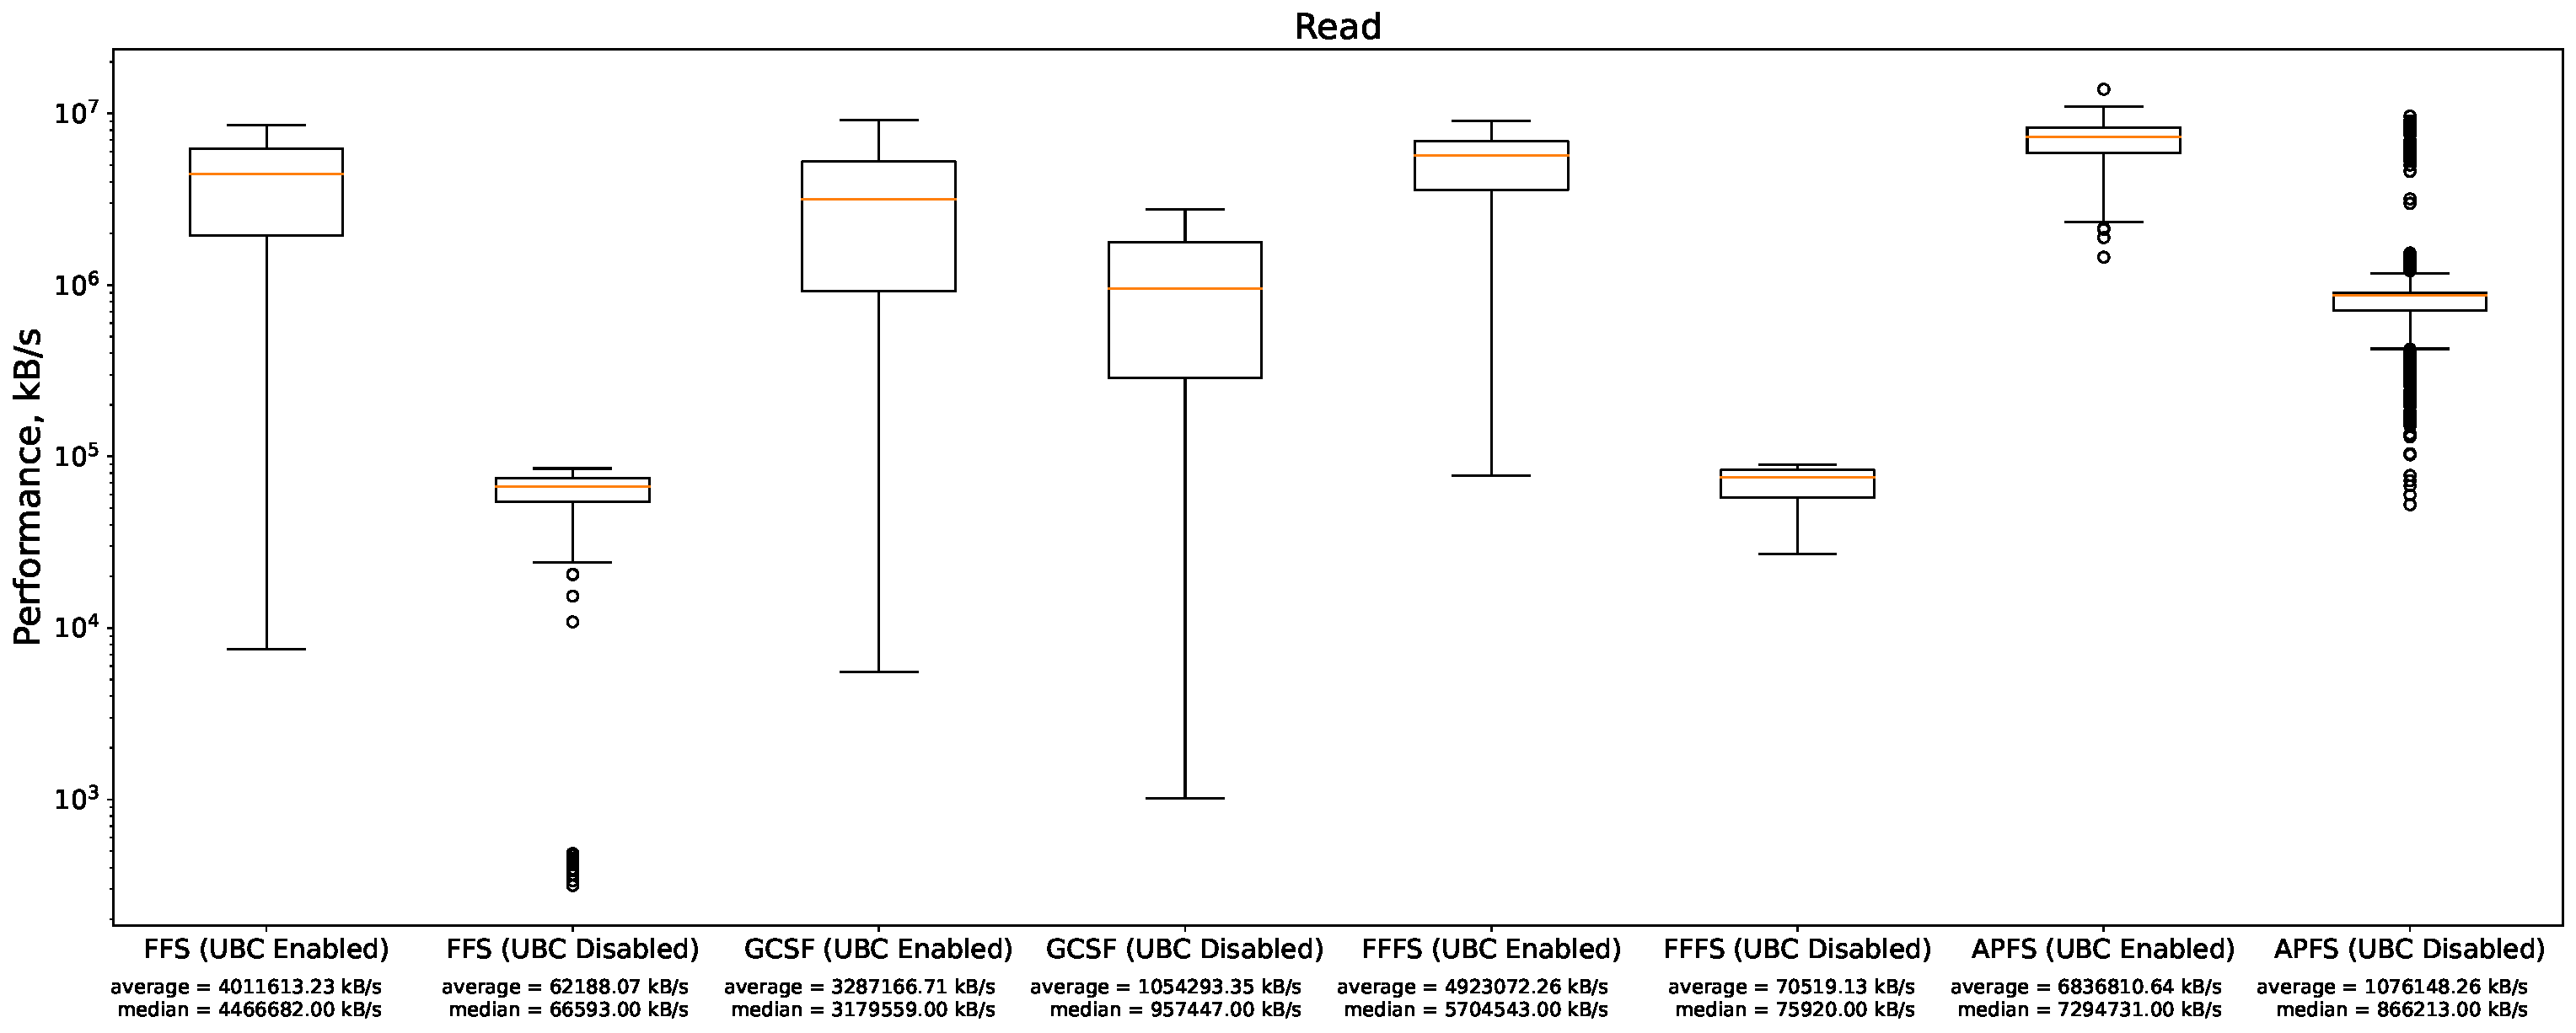
\includegraphics[width=1.0\textwidth]{figures.nosync/benchmarking/Read-boxplot.pdf}
	\end{center}
	\caption{Box plot of the IOZone output for the Read test on the different filesystems}
\end{figure}

\FloatBarrier

Figure~\ref{fig:res_box_write} presents a box plot of the benchmarking results of the filesystems of the Write test. 
% TODO: NEW TEXT
% \gls{APFS} has the best write performance of the four filesystems, followed by \gls{FFFS}. In contrast, the cloud-based filesystems \gls{FFS} and \gls{GCSF} have the worst median write performance, with \gls{FFS} having the worst performance of the filesystems. Comparing with the results of the Read test presented in Figure~\ref{fig:res_box_read}, it can also be noted that the write performance is significantly worse for the read operations for all filesystems. The average performance of the Write test for \gls{APFS} is 9.8\% of the Read performance. For \gls{FFFS}, \gls{GCSF}, and \gls{FFS} this percentage was 0.29\%, 0.17\%, and 0.06\%, respectively.

\begin{figure}[!ht]
	\label{fig:res_box_write}
	\begin{center}
		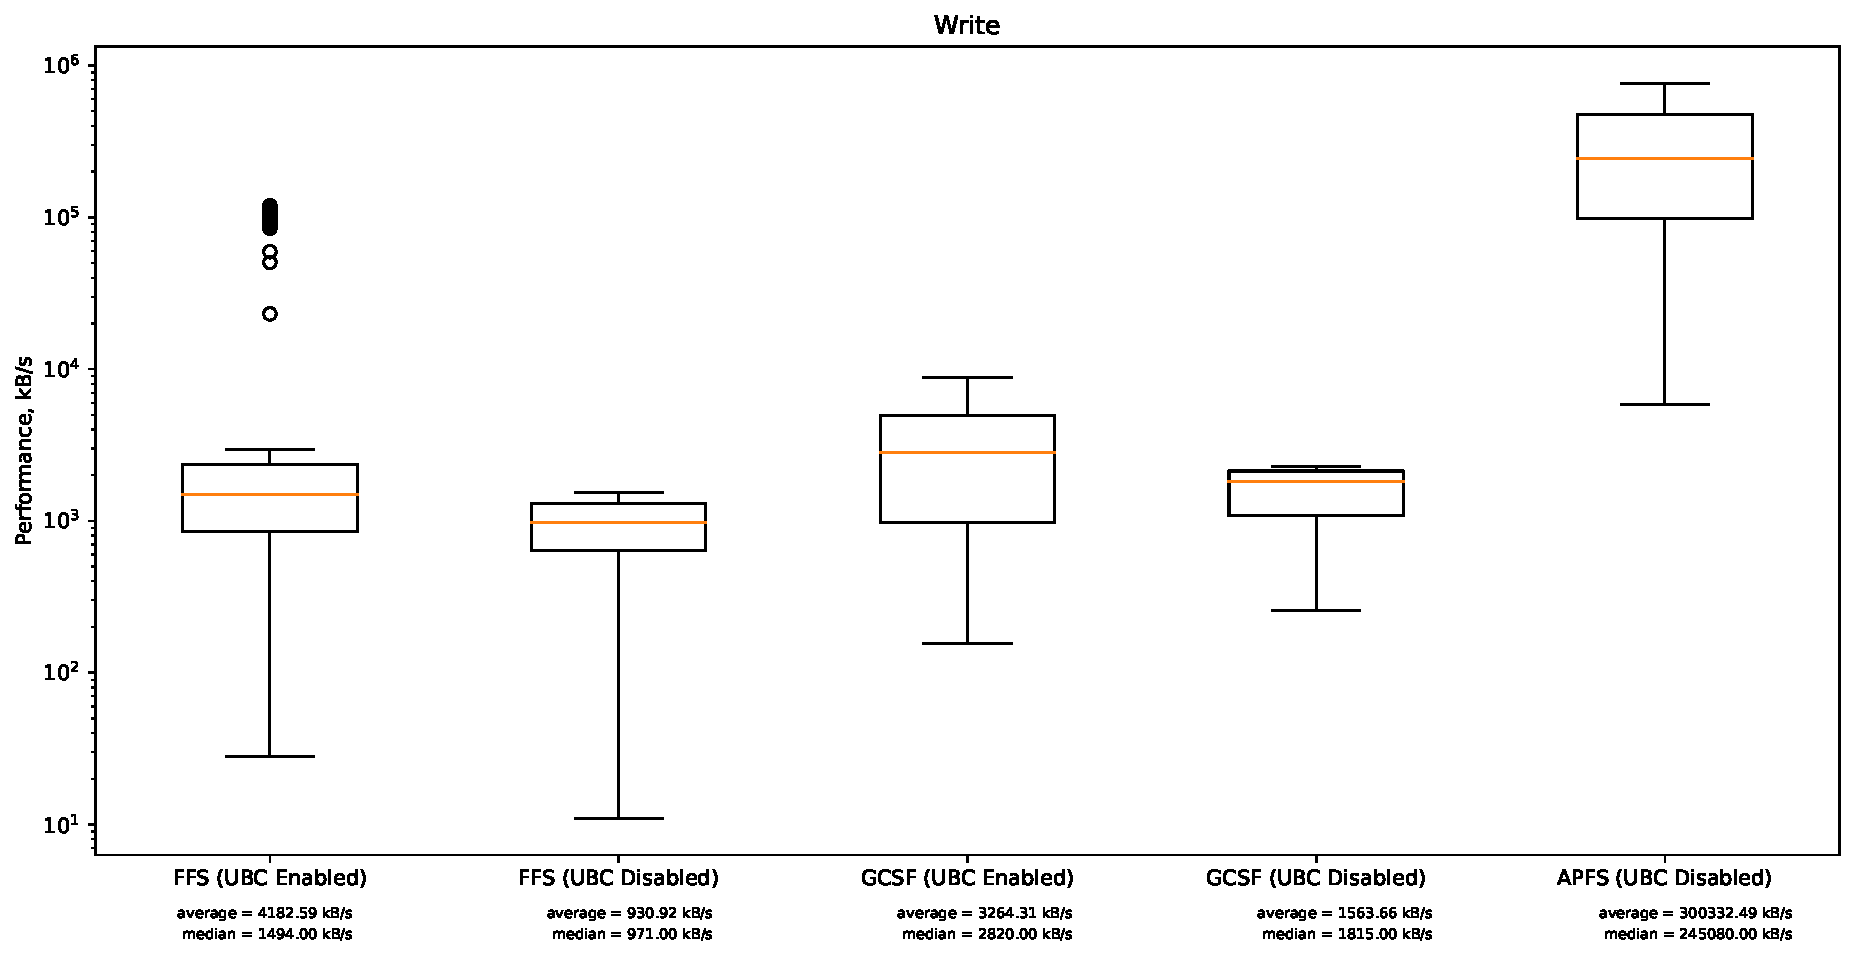
\includegraphics[width=1.0\textwidth]{figures.nosync/benchmarking/Write-boxplot.pdf}
	\end{center}
	\caption{Box plot of the IOZone output for the Write test on the different filesystems}
\end{figure}

\FloatBarrier

Figure~\ref{fig:res_box_reread} presents the result of the \mbox{Re-Read} test for the filesystems. 
%TODO: NEW TEXT
% The median performance of the filesystems are similar, with the performance of \gls{FFS} being lowest. The spread of the values for \gls{APFS} is greater than for the other filesystems but the filesystem still has the best median and average performance. While the average performance for the Re-Read test of \gls{APFS} is around \SI[per-mode = symbol]{5\,400\,000}{\kilo\byte\per\second}, the lowest performance was at \SI[per-mode = symbol]{422\,414}{\kilo\byte\per\second}, namely for \texttt{file size = 32\,768\,kB, buffer size = 8\,kB}. The spread of values is higher for \gls{FFS} than for \gls{FFFS} and \gls{GCSF}. \gls{FFFS} has a higher average and median performance than \gls{GCSF}.

\begin{figure}[!ht]
	\label{fig:res_box_reread}
	\begin{center}
		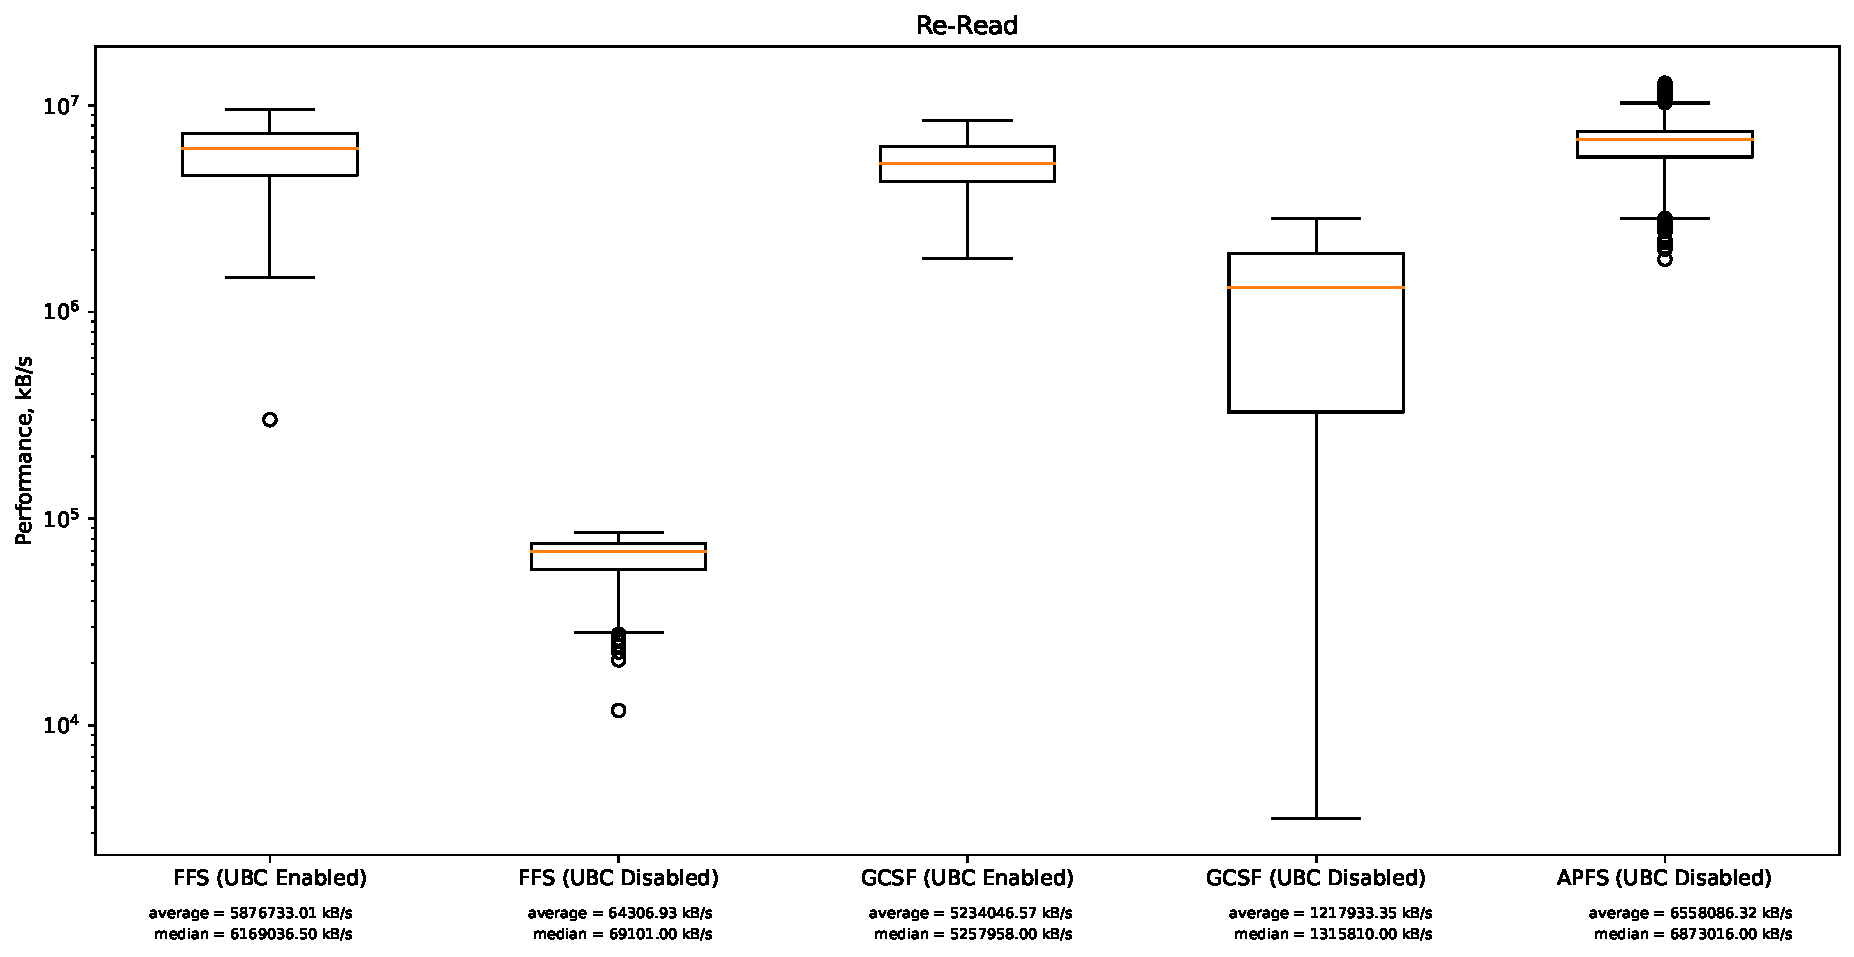
\includegraphics[width=1.0\textwidth]{figures.nosync/benchmarking/Re-Read-boxplot.pdf}
	\end{center}
	\caption{Box plot of the IOZone output for the Re-Read test on the different filesystems}
\end{figure}

\FloatBarrier

Figure~\ref{fig:res_box_rewrite} presents a box plot for the \mbox{Re-Write} test for the filesystems. 
%TODO: NEW TEXT
% Similar to the Write test results presented in Figure~\ref{fig:res_box_write}, \gls{APFS} has the best performance of the filesystems, followed by \gls{FFFS} and finally the two cloud-based filesystems. \gls{APFS} is the only filesystem that has a higher average and median performance for the \mbox{Re-Write} test compared to its Write test, with a 22\% better median performance. The other filesystems have worse average and median performance for the \mbox{Re-Write} compared to their Write test. The median performance of the \mbox{Re-Write} test for \gls{FFS}, \gls{FFFS}, and \gls{GCSF} are 85\%, 82\%, and 64\% of the median performance of their Write test, respectively. 

\begin{figure}[!ht]
	\label{fig:res_box_rewrite}
	\begin{center}
		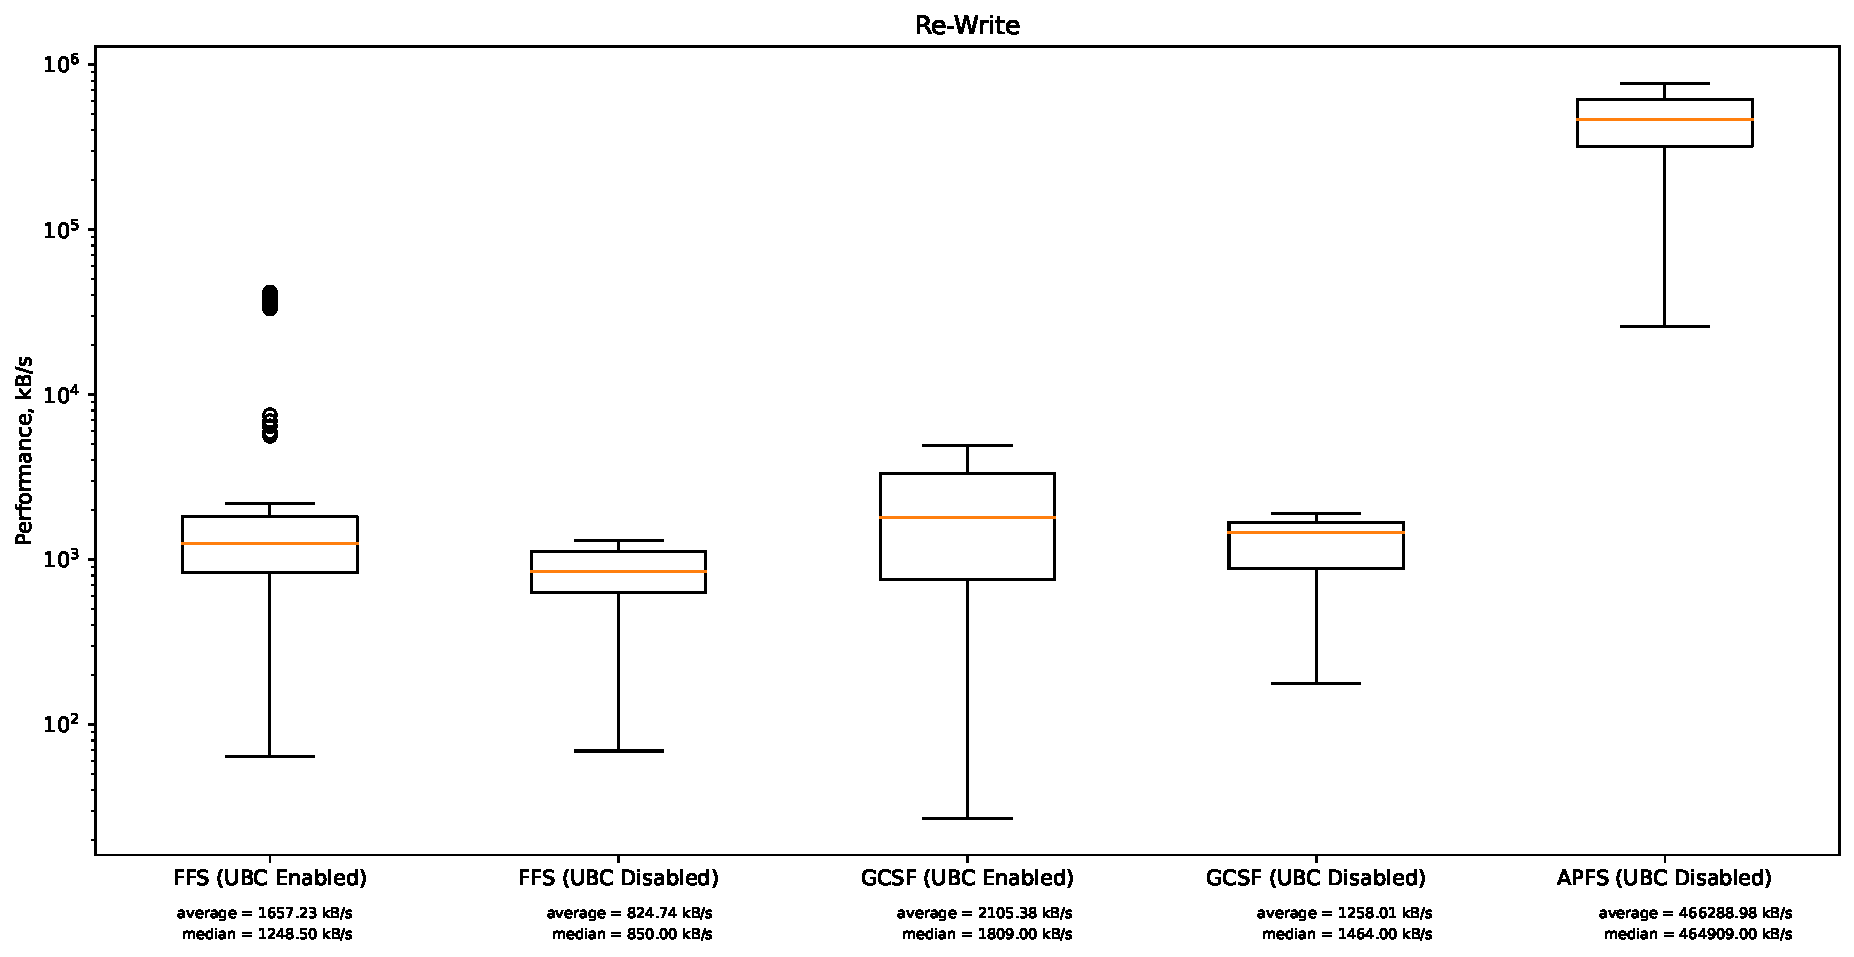
\includegraphics[width=1.0\textwidth]{figures.nosync/benchmarking/Re-Write-boxplot.pdf}
	\end{center}
	\caption{Box plot of the IOZone output for the Re-Write test on the different filesystems}
\end{figure}

\FloatBarrier

Figure~\ref{fig:res_box_rndread} presents a box plot for the Random read test for the different filesystems. 
% TODO: NEW TEXT
% The results are similar to the results for the \mbox{Re-Read} test presented in Figure~\ref{fig:res_box_reread}, however, \gls{FFS} has a bigger spread of values than \gls{APFS} has in the \mbox{Re-Read} test. \gls{FFFS} has the best average performance of the filesystems, and \gls{APFS} has the best median performance. The median and average performance of \gls{FFS} is lower than the other filesystems.

\begin{figure}[!ht]
	\label{fig:res_box_rndread}
	\begin{center}
		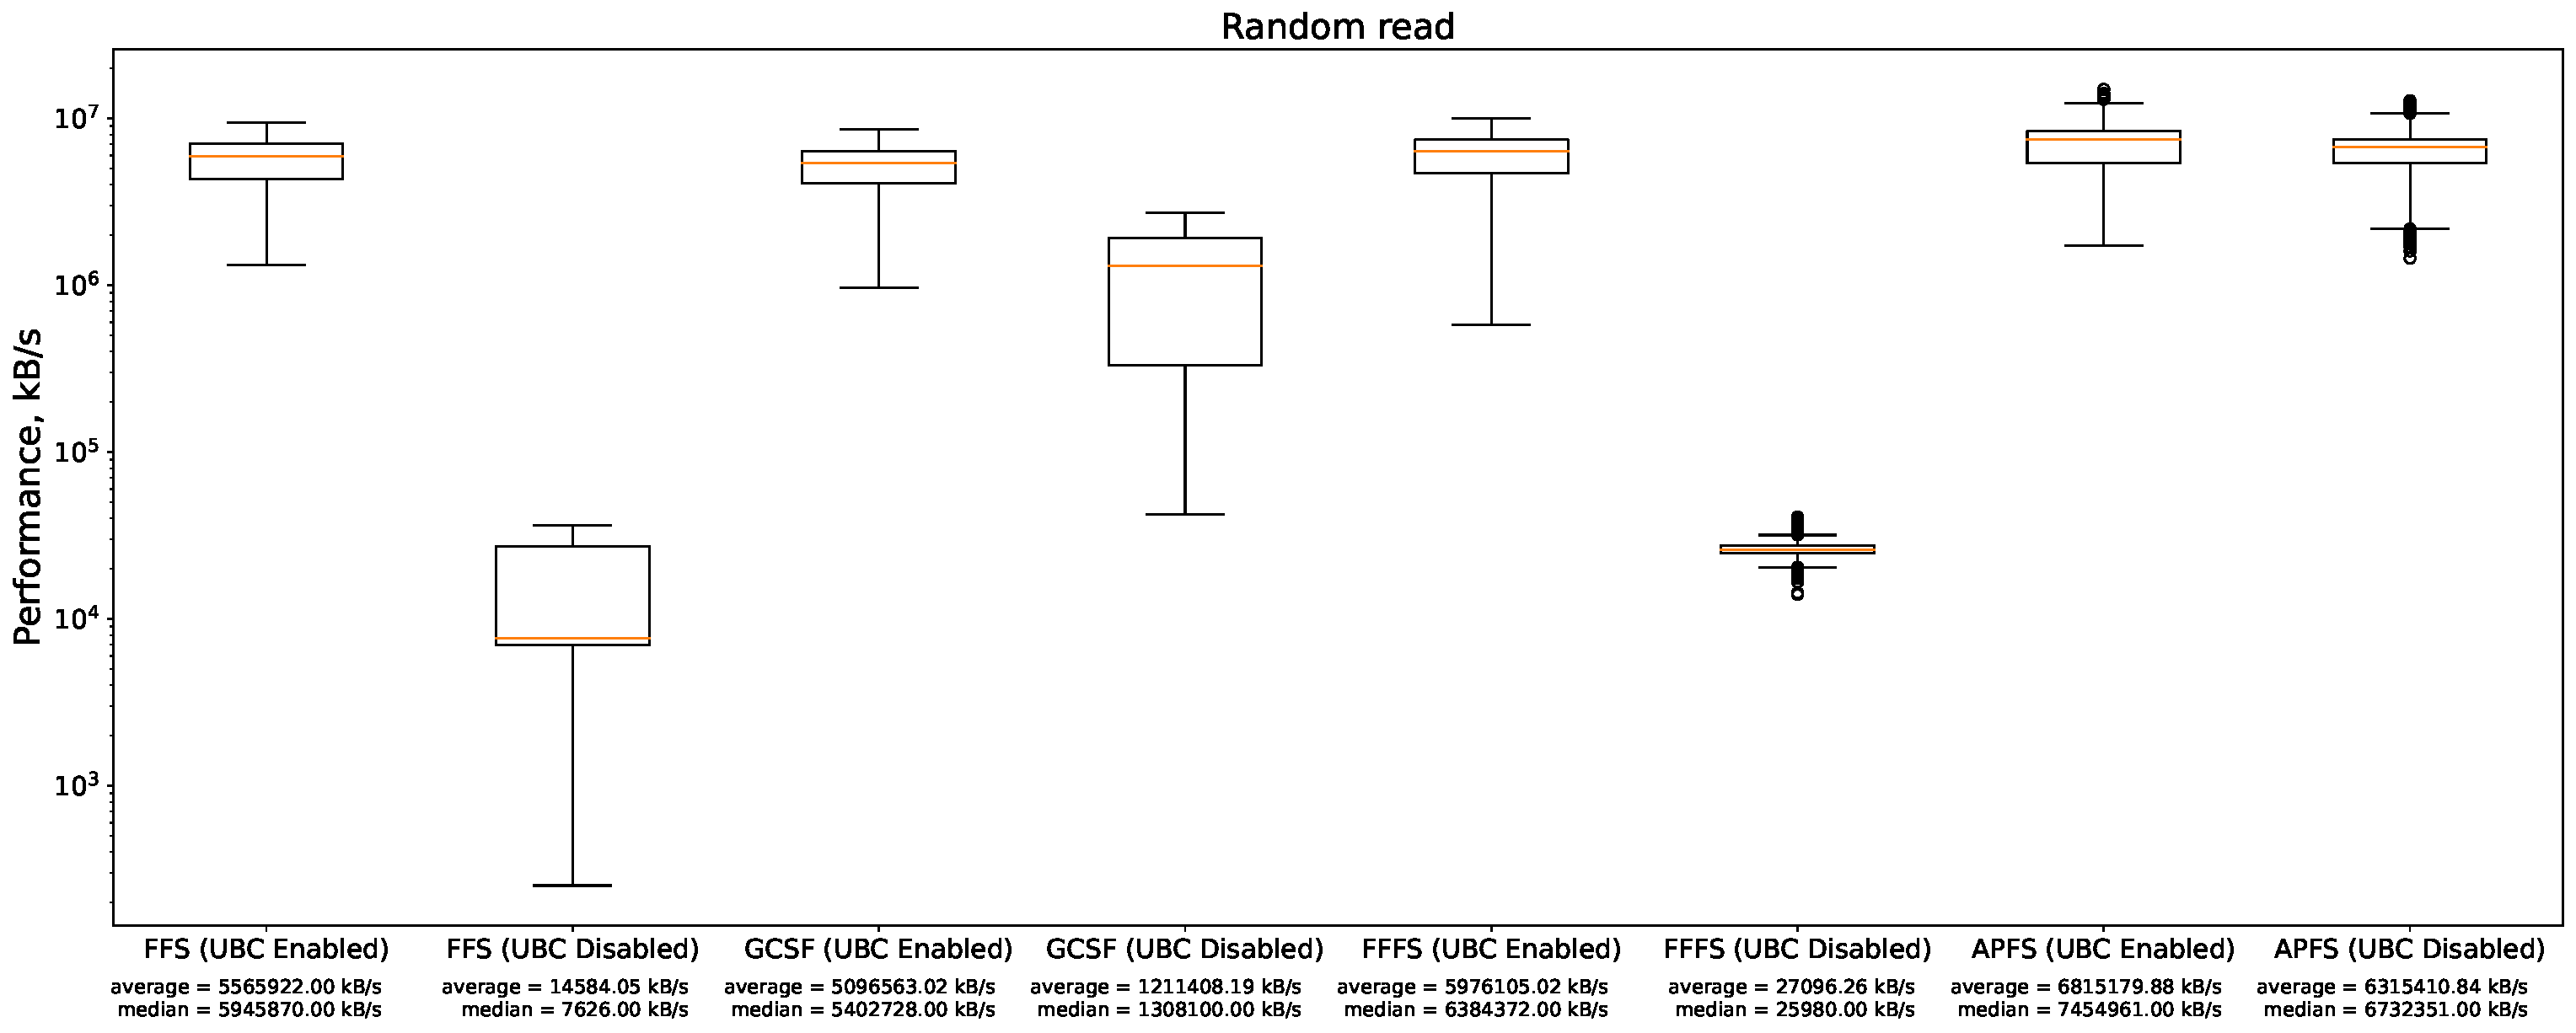
\includegraphics[width=1.0\textwidth]{figures.nosync/benchmarking/Random read-boxplot.pdf}
	\end{center}
	\caption{Box plot of the IOZone output for the Random read test on the different filesystems}
\end{figure}

\FloatBarrier

Figure~\ref{fig:res_box_rndwrite} presents a box plot for the Random read test for the different filesystems. 
% TODO: New text
%\gls{APFS} has the highest performance, followed by \gls{FFFS} and the cloud-based filesystems. \gls{GCSF} has better performance than \gls{FFS}. The performances are similar to the \mbox{Re-Write} for all filesystems.

\begin{figure}[!ht]
	\label{fig:res_box_rndwrite}
	\begin{center}
		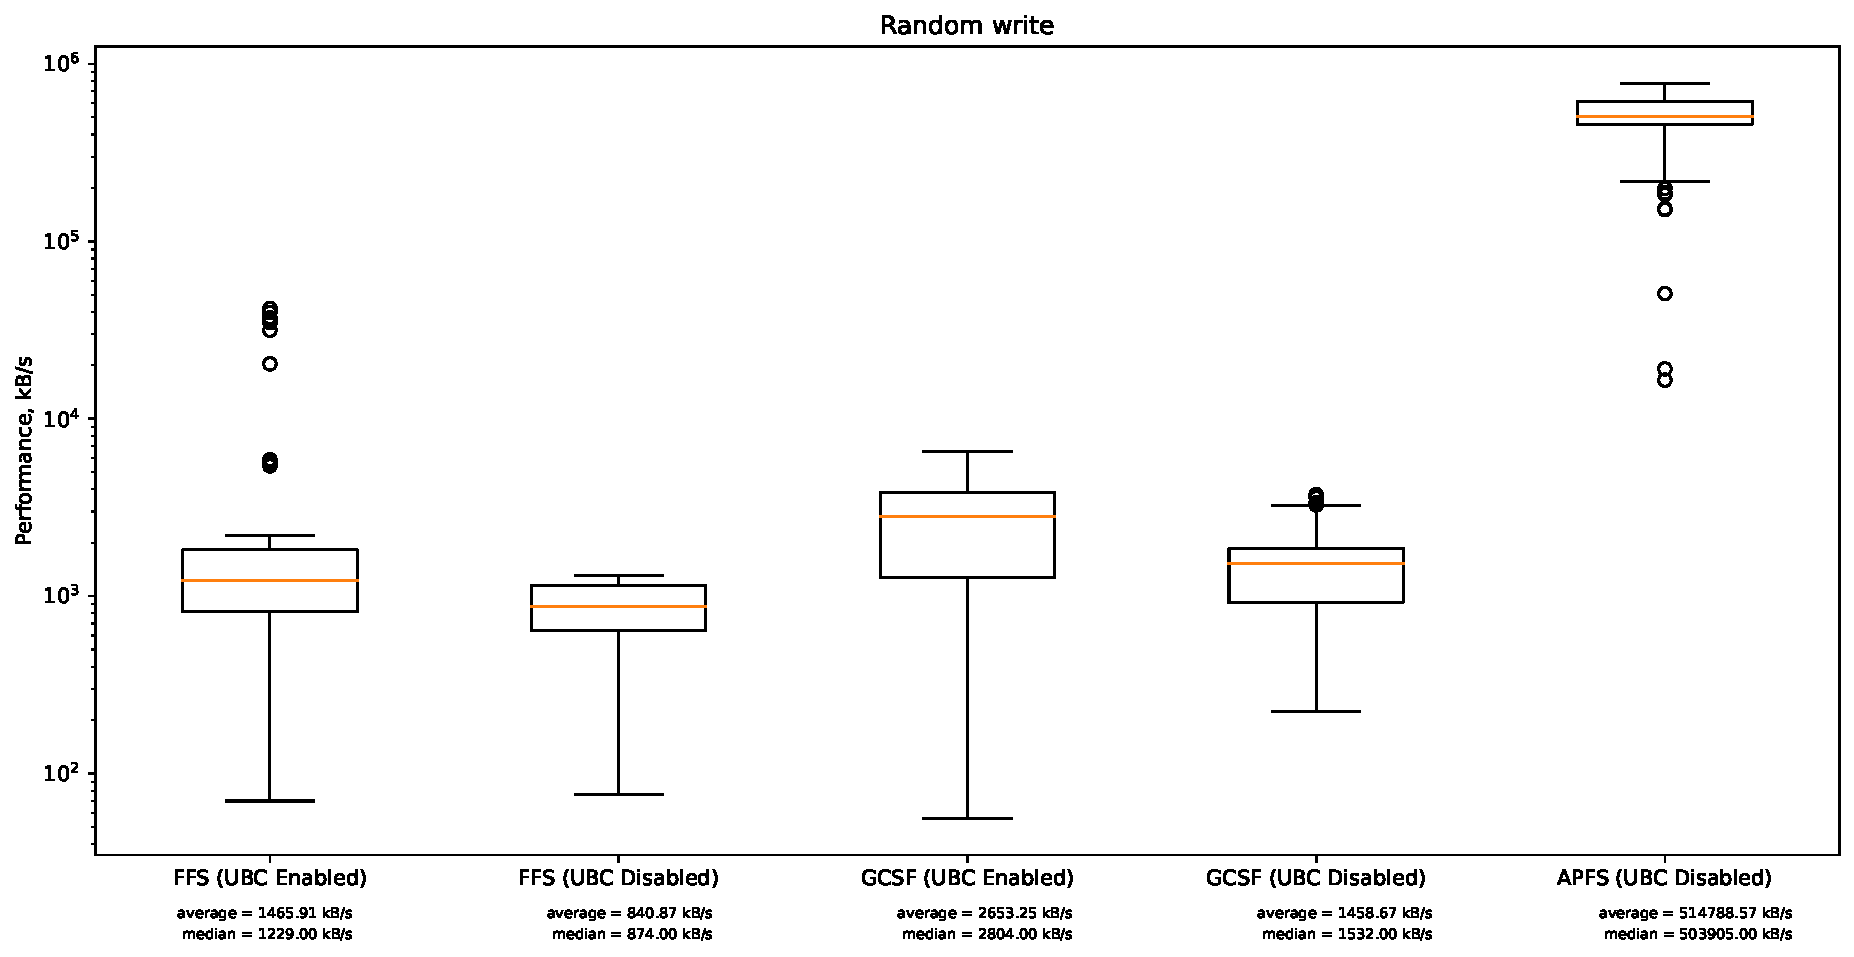
\includegraphics[width=1.0\textwidth]{figures.nosync/benchmarking/Random write-boxplot.pdf}
	\end{center}
	\caption{Box plot of the IOZone output for the Random write test on the different filesystems}
\end{figure}

\FloatBarrier

% TODO: Fixme
\gls{FFS} does not have the best performance in any of the box plots presented. \gls{GCSF} has better performance than \gls{FFS} for all tests run with the benchmarking.
%  Following are diagrams presenting the performance of each benchmarking test per file size, for each filesystem. The raw data tables can be found in Appendix~\ref{app:bench_data}. Figure~\ref{fig:bench_ffs_read} to Figure~\ref{fig:bench_ffs_rnd_write} present the performances of the Read, Write, \mbox{Re-Read}, \mbox{Re-Write}, Random Read, and Random Write tests for \gls{FFS}. Figure~\ref{fig:bench_fffs_read} to Figure~\ref{fig:bench_fffs_rnd_write} present the performances of the Read, Write, \mbox{Re-Read}, \mbox{Re-Write}, Random Read, and Random Write tests for \gls{FFFS}.  Figure~\ref{fig:bench_gcsf_read} to Figure~\ref{fig:bench_gcsf_rnd_write} present the performances of the Read, Write, \mbox{Re-Read}, \mbox{Re-Write}, Random Read, and Random Write tests for \gls{GCSF}. Figure~\ref{fig:bench_apfs_read} to Figure~\ref{fig:bench_apfs_rnd_write} present the performances of the Read, Write, \mbox{Re-Read}, \mbox{Re-Write}, Random Read, and Random Write tests for \gls{APFS}.



\begin{figure}[!htb]
	\label{fig:bench_ffs_with_cache}
	\begin{center}
		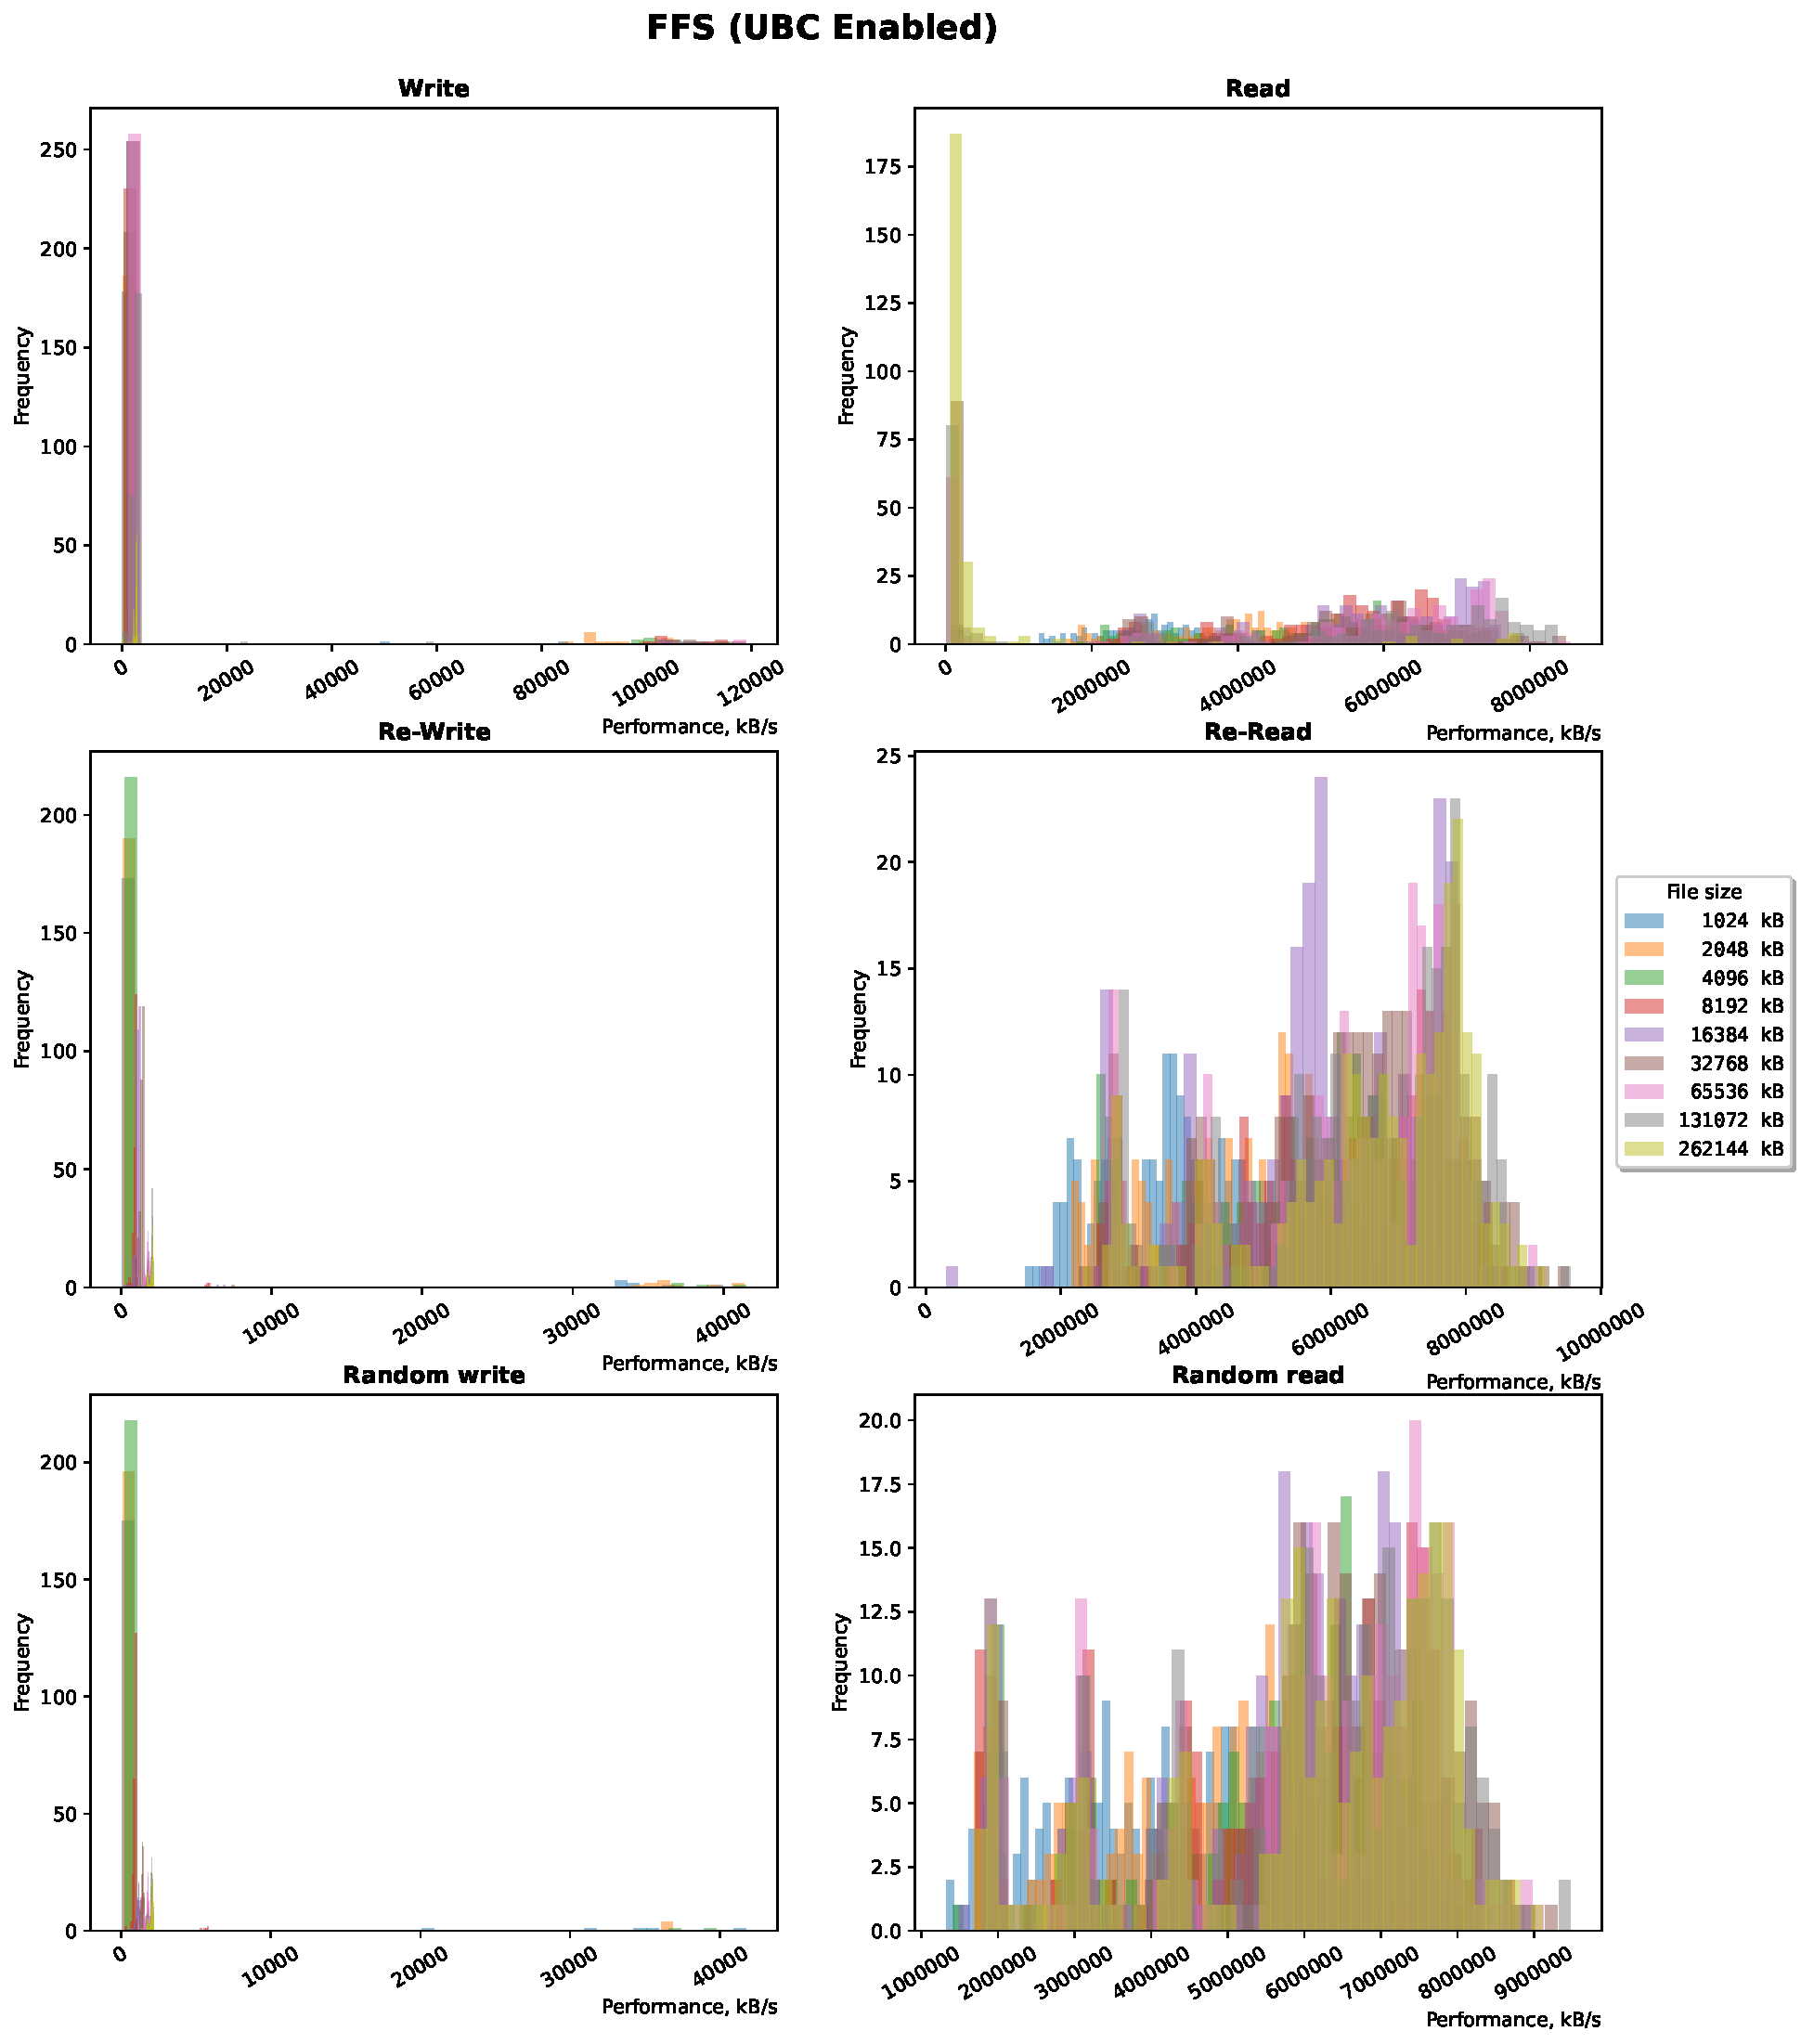
\includegraphics[width=1.0\textwidth]{figures.nosync/benchmarking/FFS/FFS-UBC Enabled-hist.pdf}
	\end{center}
	\caption{Performance comparison of different file sizes for FFS with the UBC enabled}
\end{figure}

\begin{figure}[!htb]
	\label{fig:bench_ffs_without_cache}
	\begin{center}
		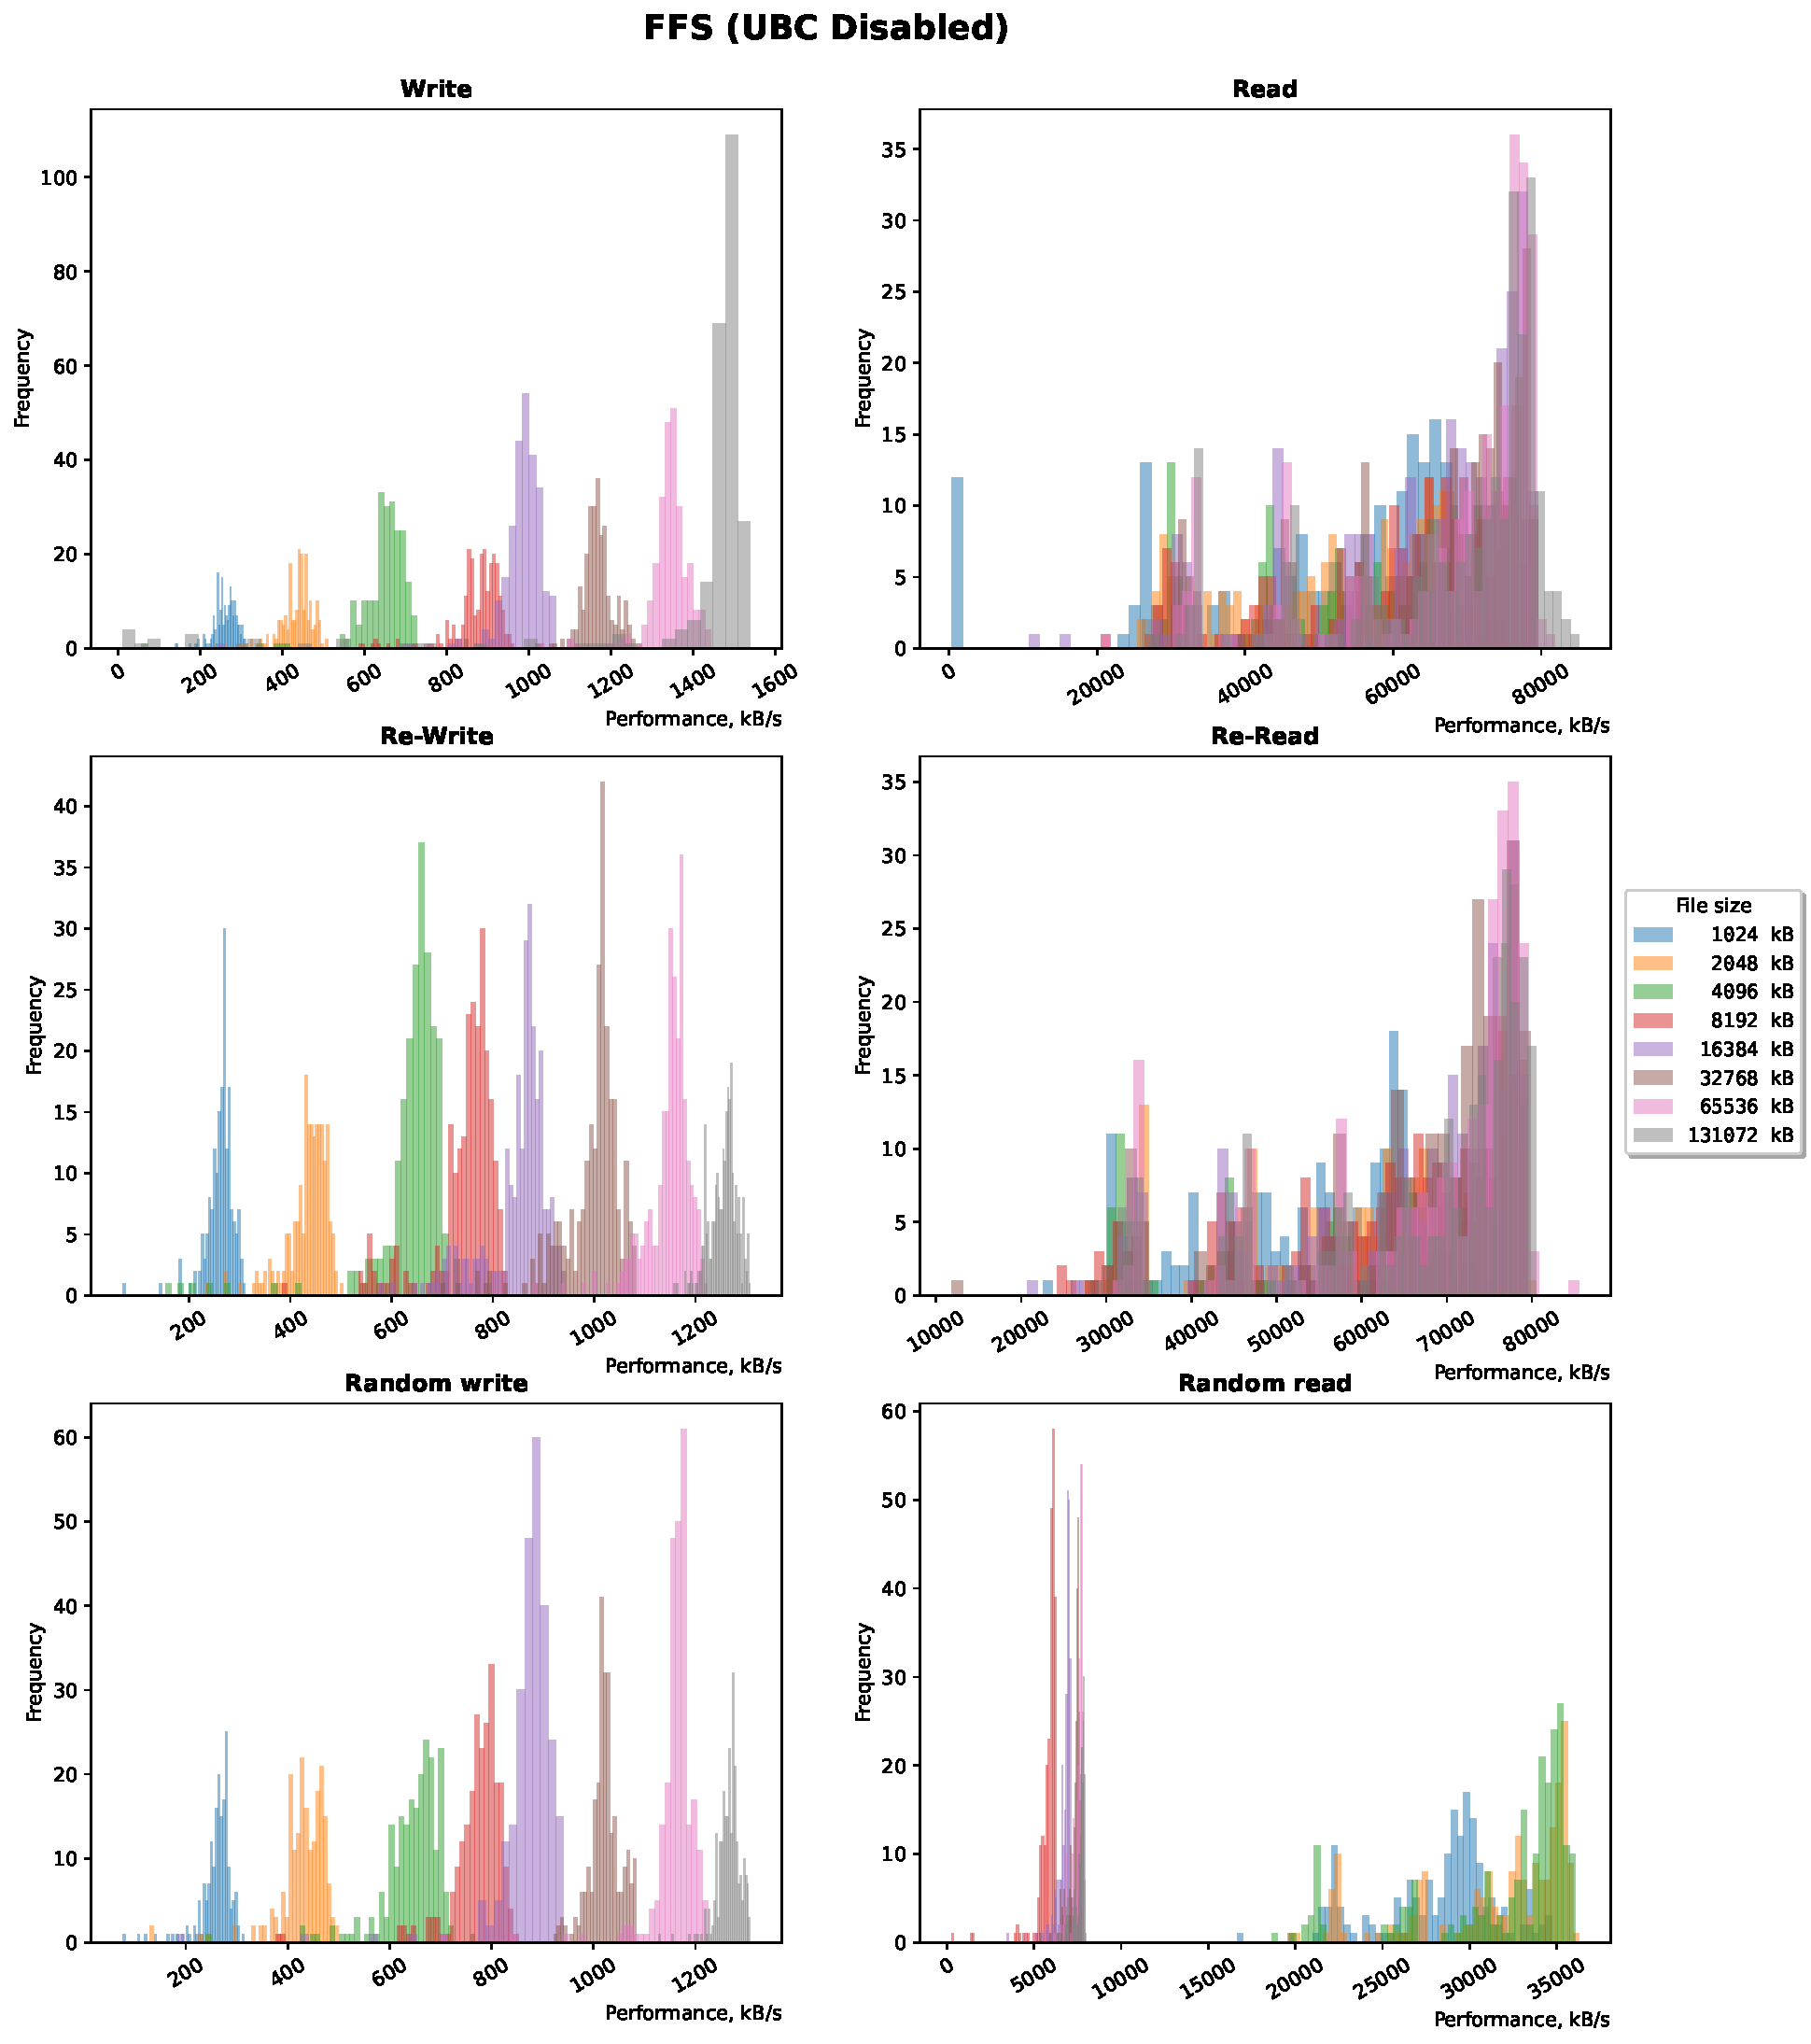
\includegraphics[width=1.0\textwidth]{figures.nosync/benchmarking/FFS/FFS-UBC Disabled-hist.pdf}
	\end{center}
	\caption{Performance comparison of different file sizes for FFS with the UBC disabled}
\end{figure}



\begin{figure}[!htb]
	\label{fig:bench_gcsf_with_cache}
	\begin{center}
		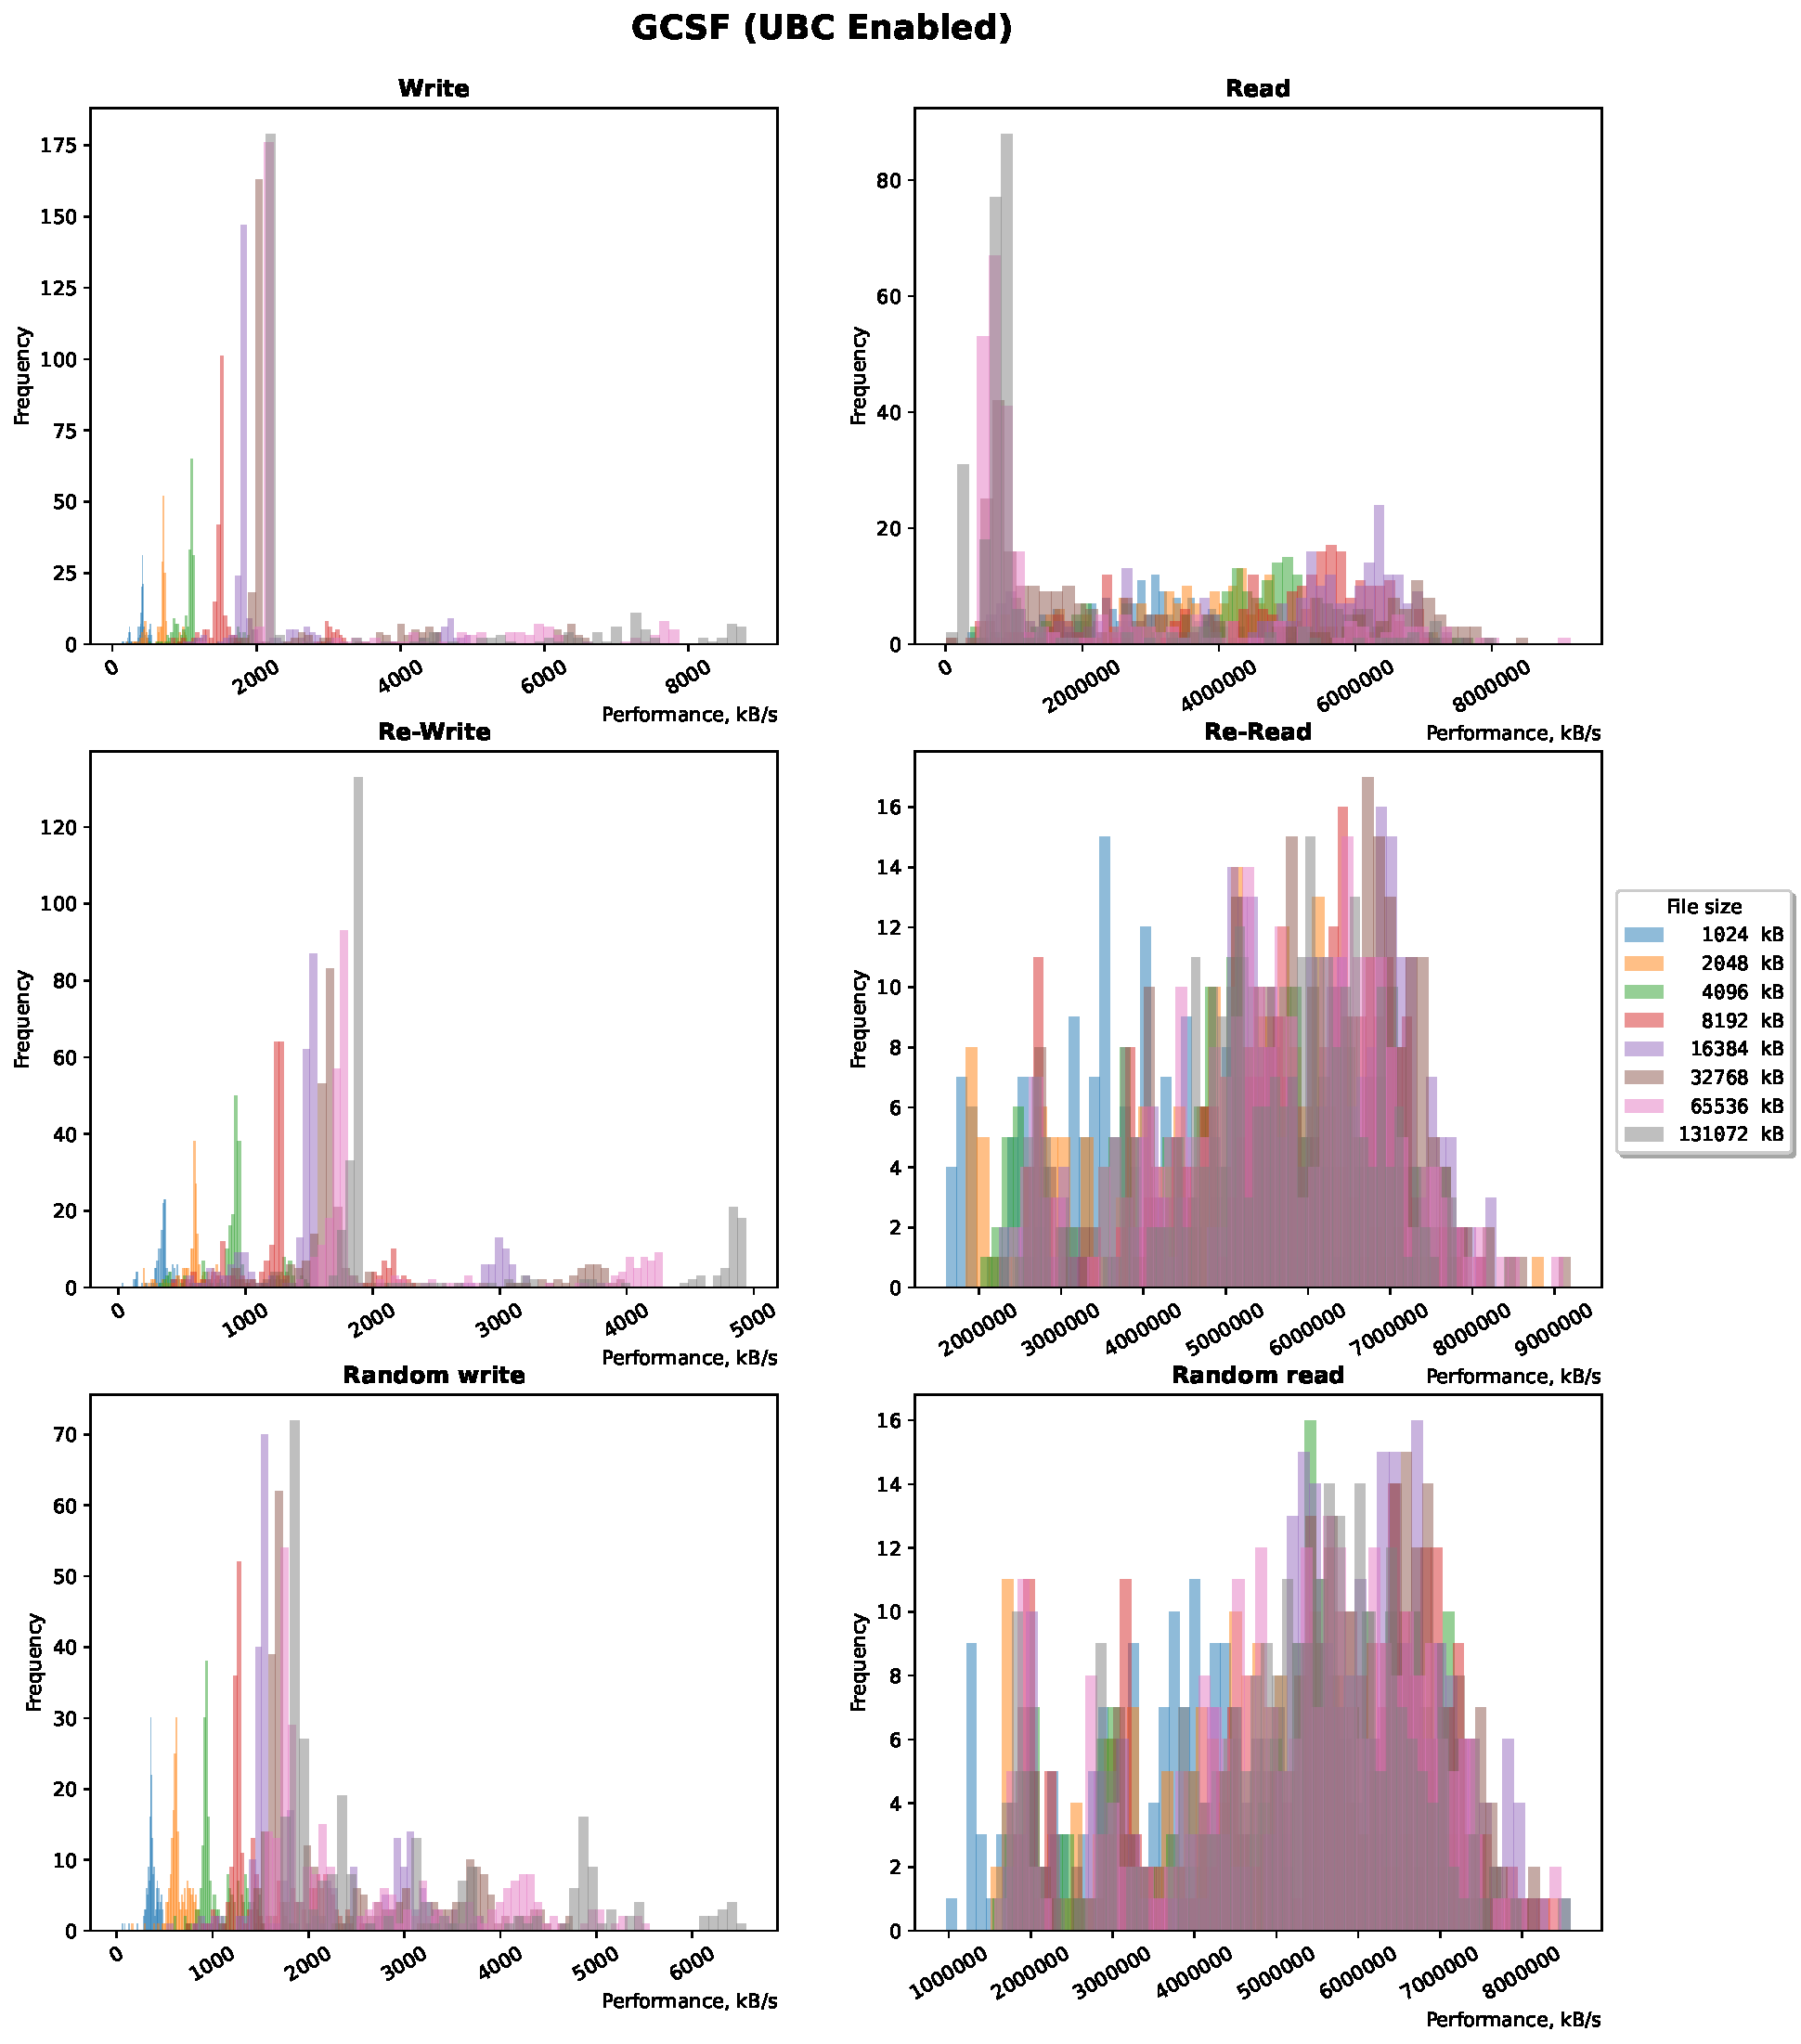
\includegraphics[width=1.0\textwidth]{figures.nosync/benchmarking/GCSF/GCSF-UBC Enabled-hist.pdf}
	\end{center}
	\caption{Performance comparison of different file sizes for GCSF with the UBC enabled}
\end{figure}

\begin{figure}[!htb]
	\label{fig:bench_gcsf_without_cache}
	\begin{center}
		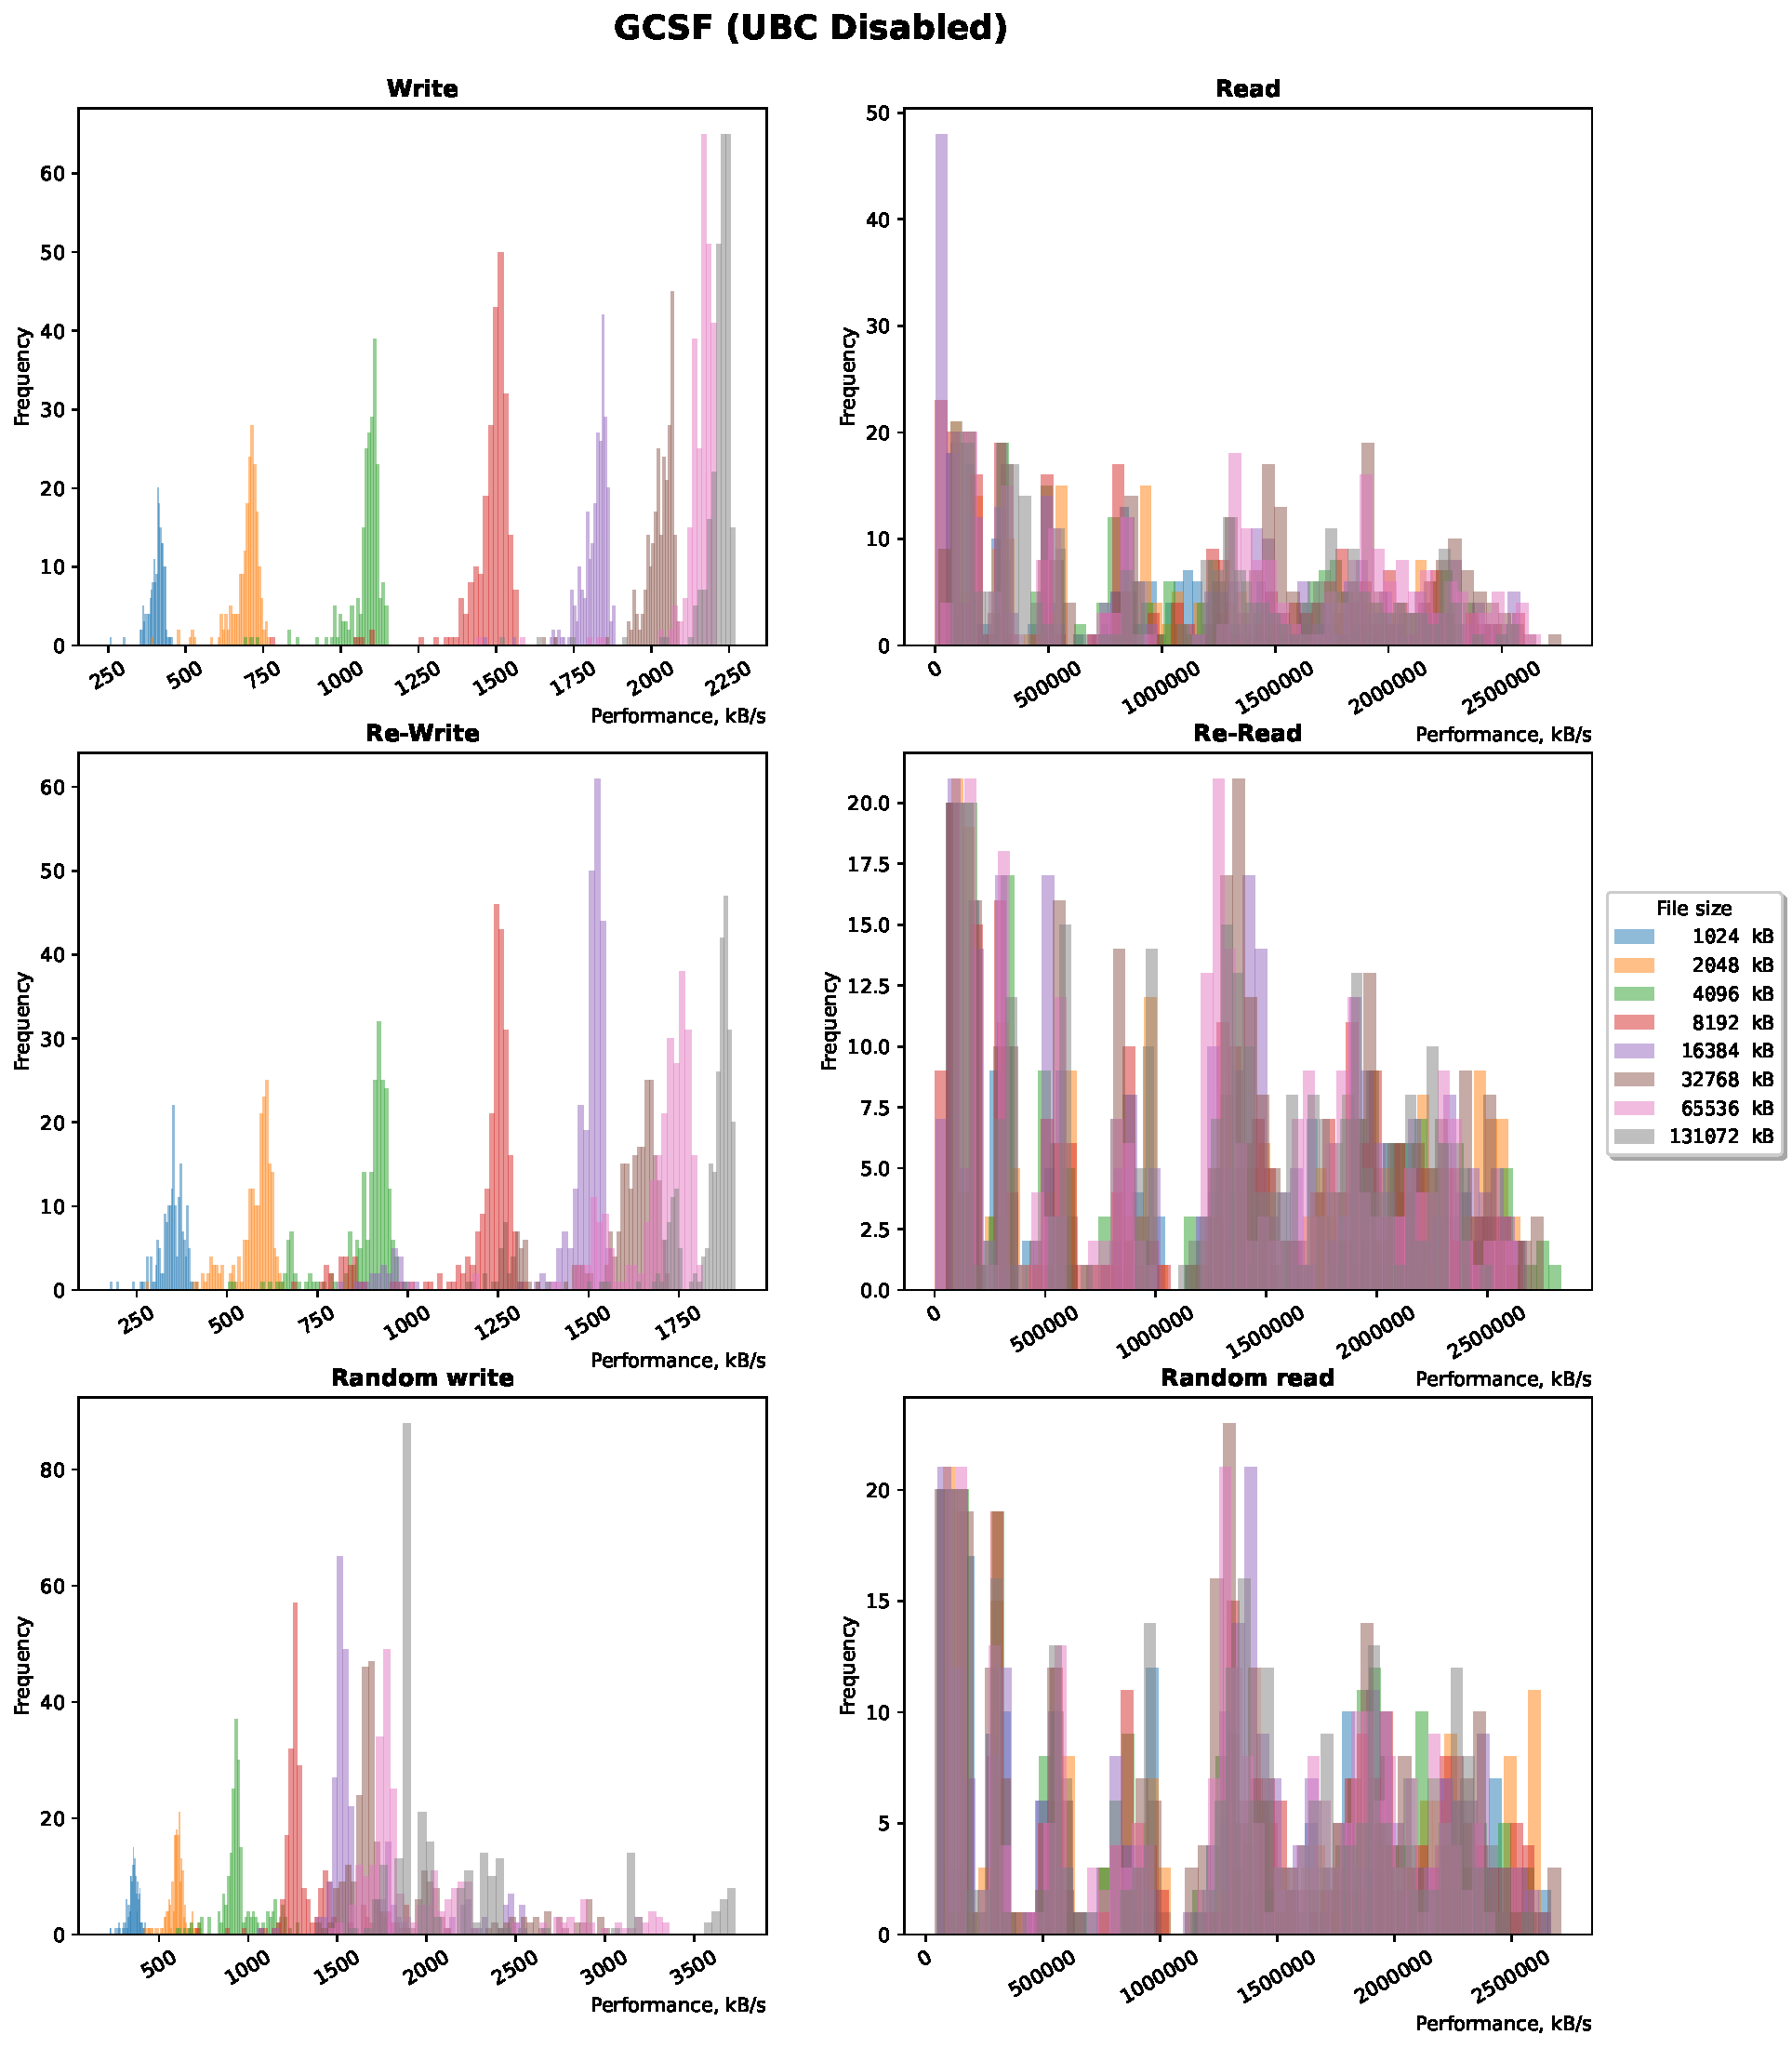
\includegraphics[width=1.0\textwidth]{figures.nosync/benchmarking/GCSF/GCSF-UBC Disabled-hist.pdf}
	\end{center}
	\caption{Performance comparison of different file sizes for GCSF with the UBC disabled}
\end{figure}


\begin{figure}[!htb]
	\label{fig:bench_fffs_with_cache}
	\begin{center}
		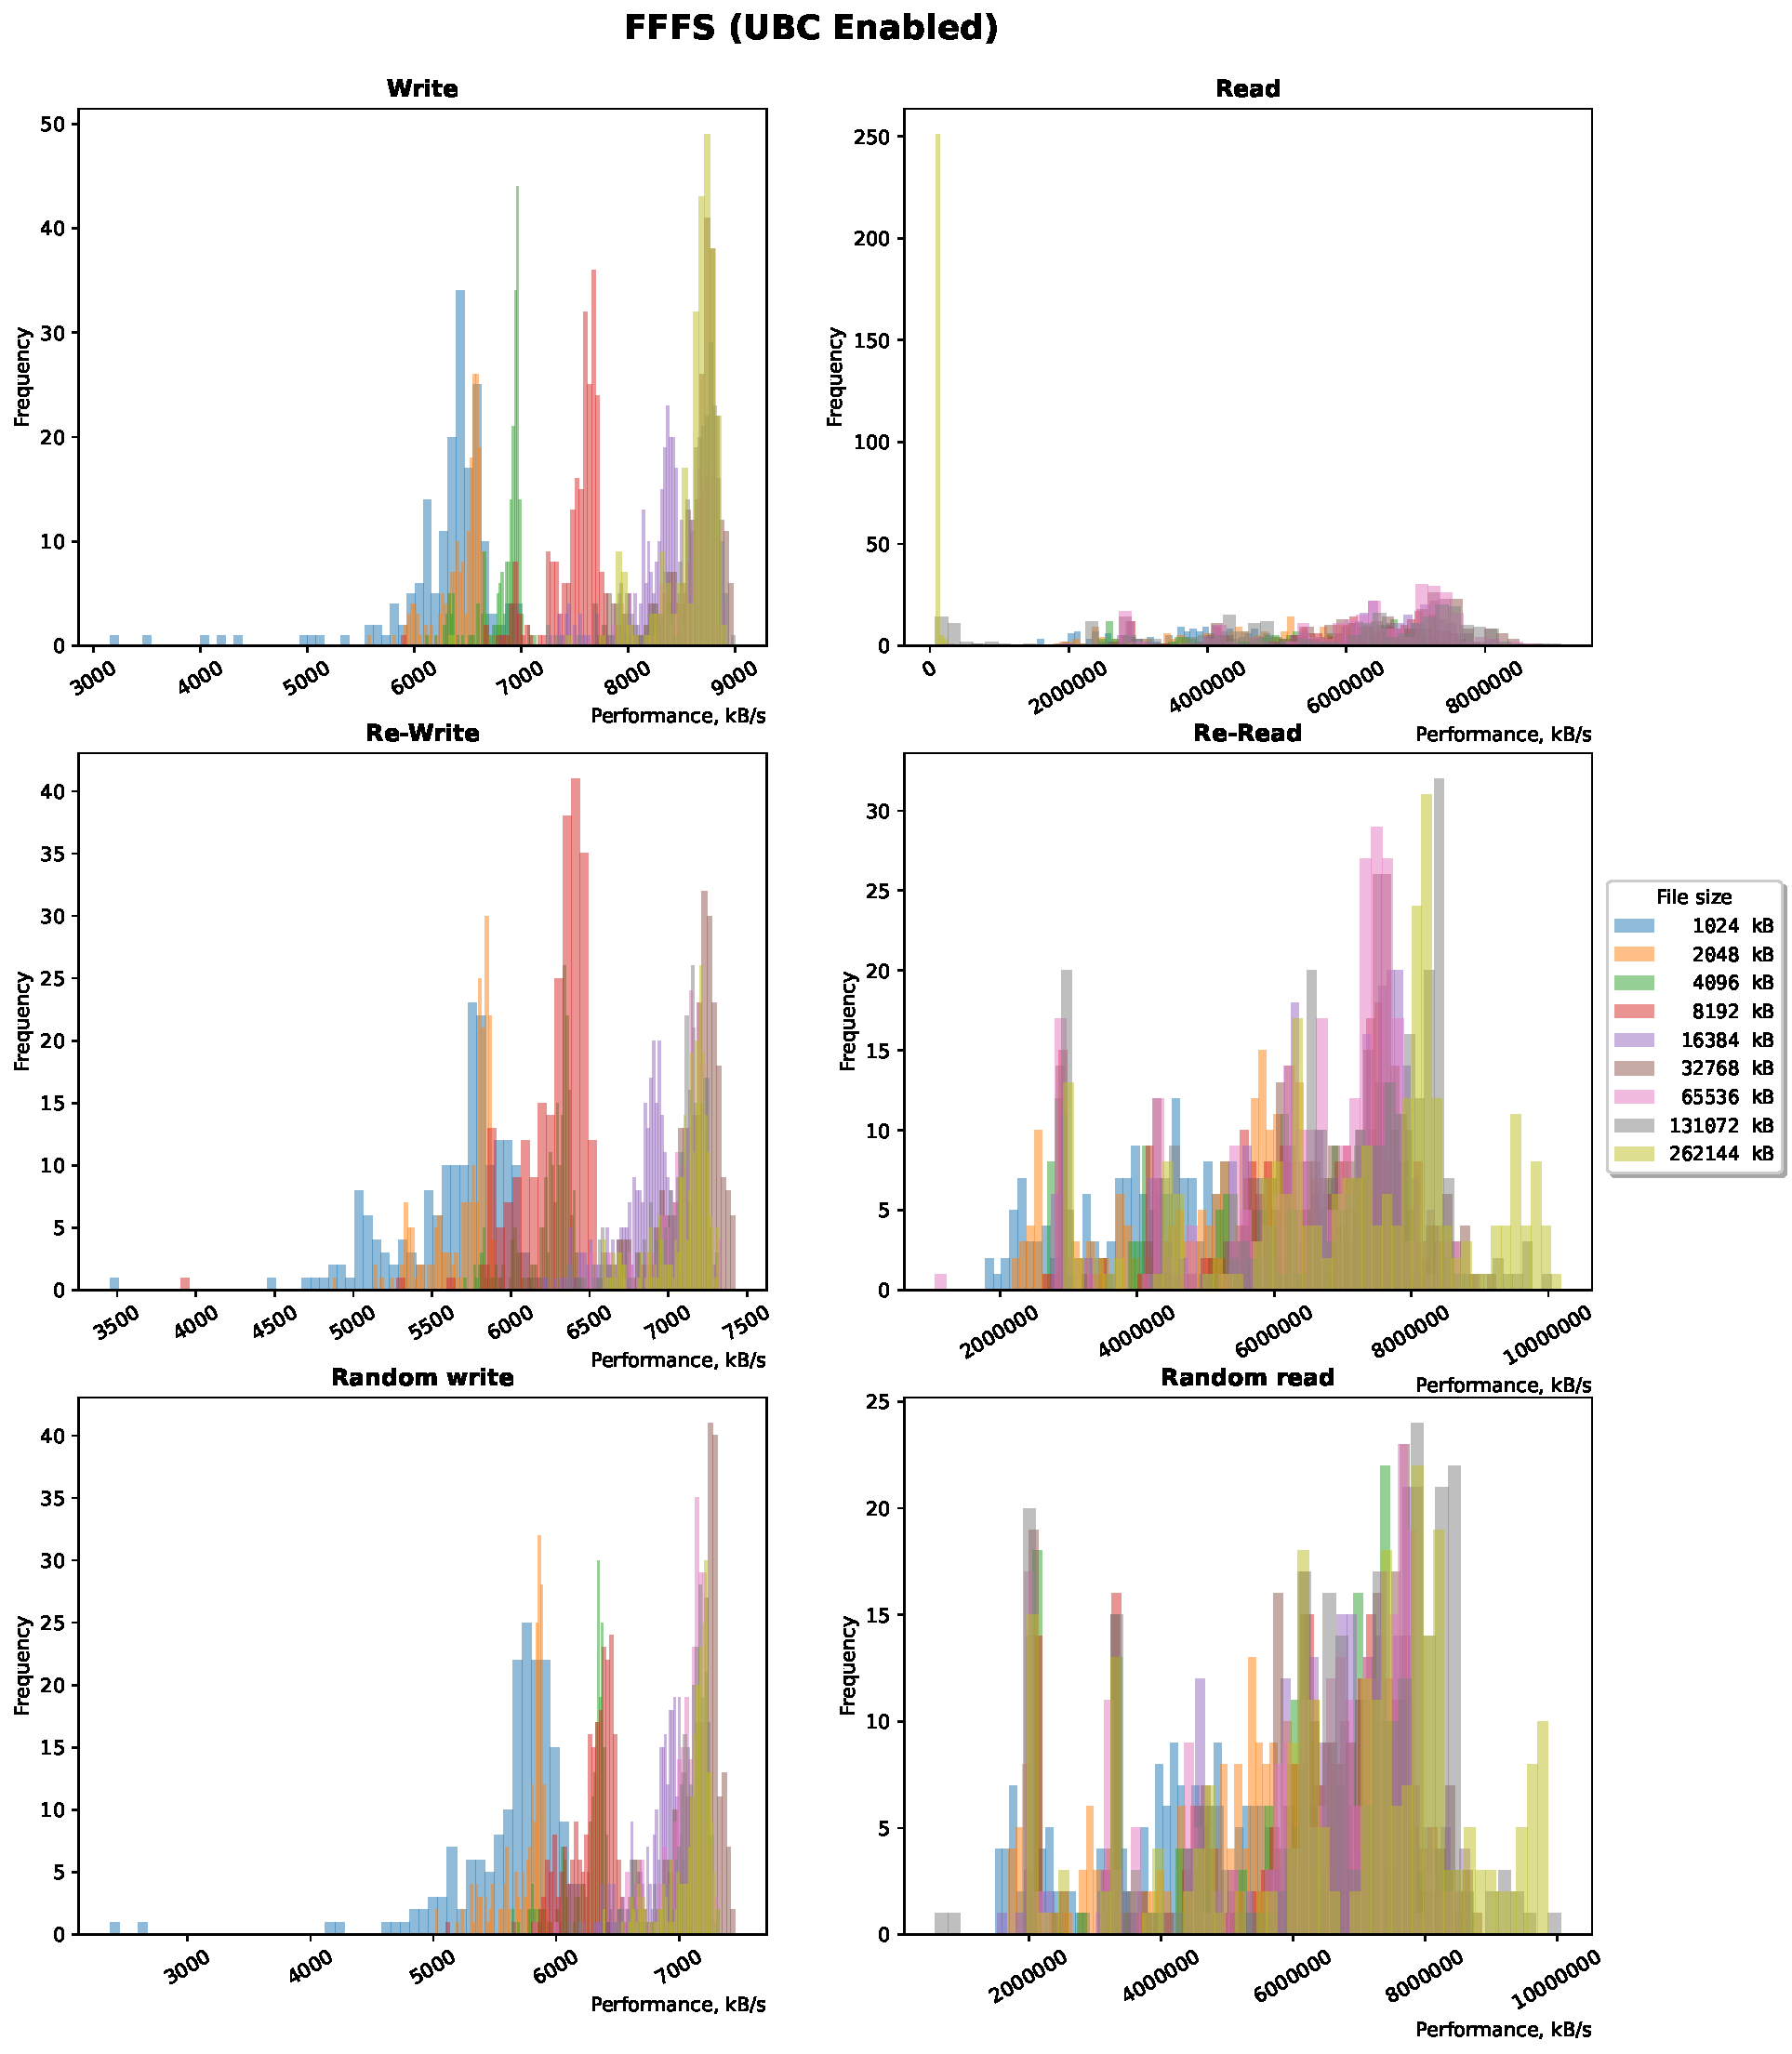
\includegraphics[width=1.0\textwidth]{figures.nosync/benchmarking/FFFS/FFFS-UBC Enabled-hist.pdf}
	\end{center}
	\caption{Performance comparison of different file sizes for FFFS with the UBC enabled}
\end{figure}

\begin{figure}[!htb]
	\label{fig:bench_fffs_without_cache}
	\begin{center}
		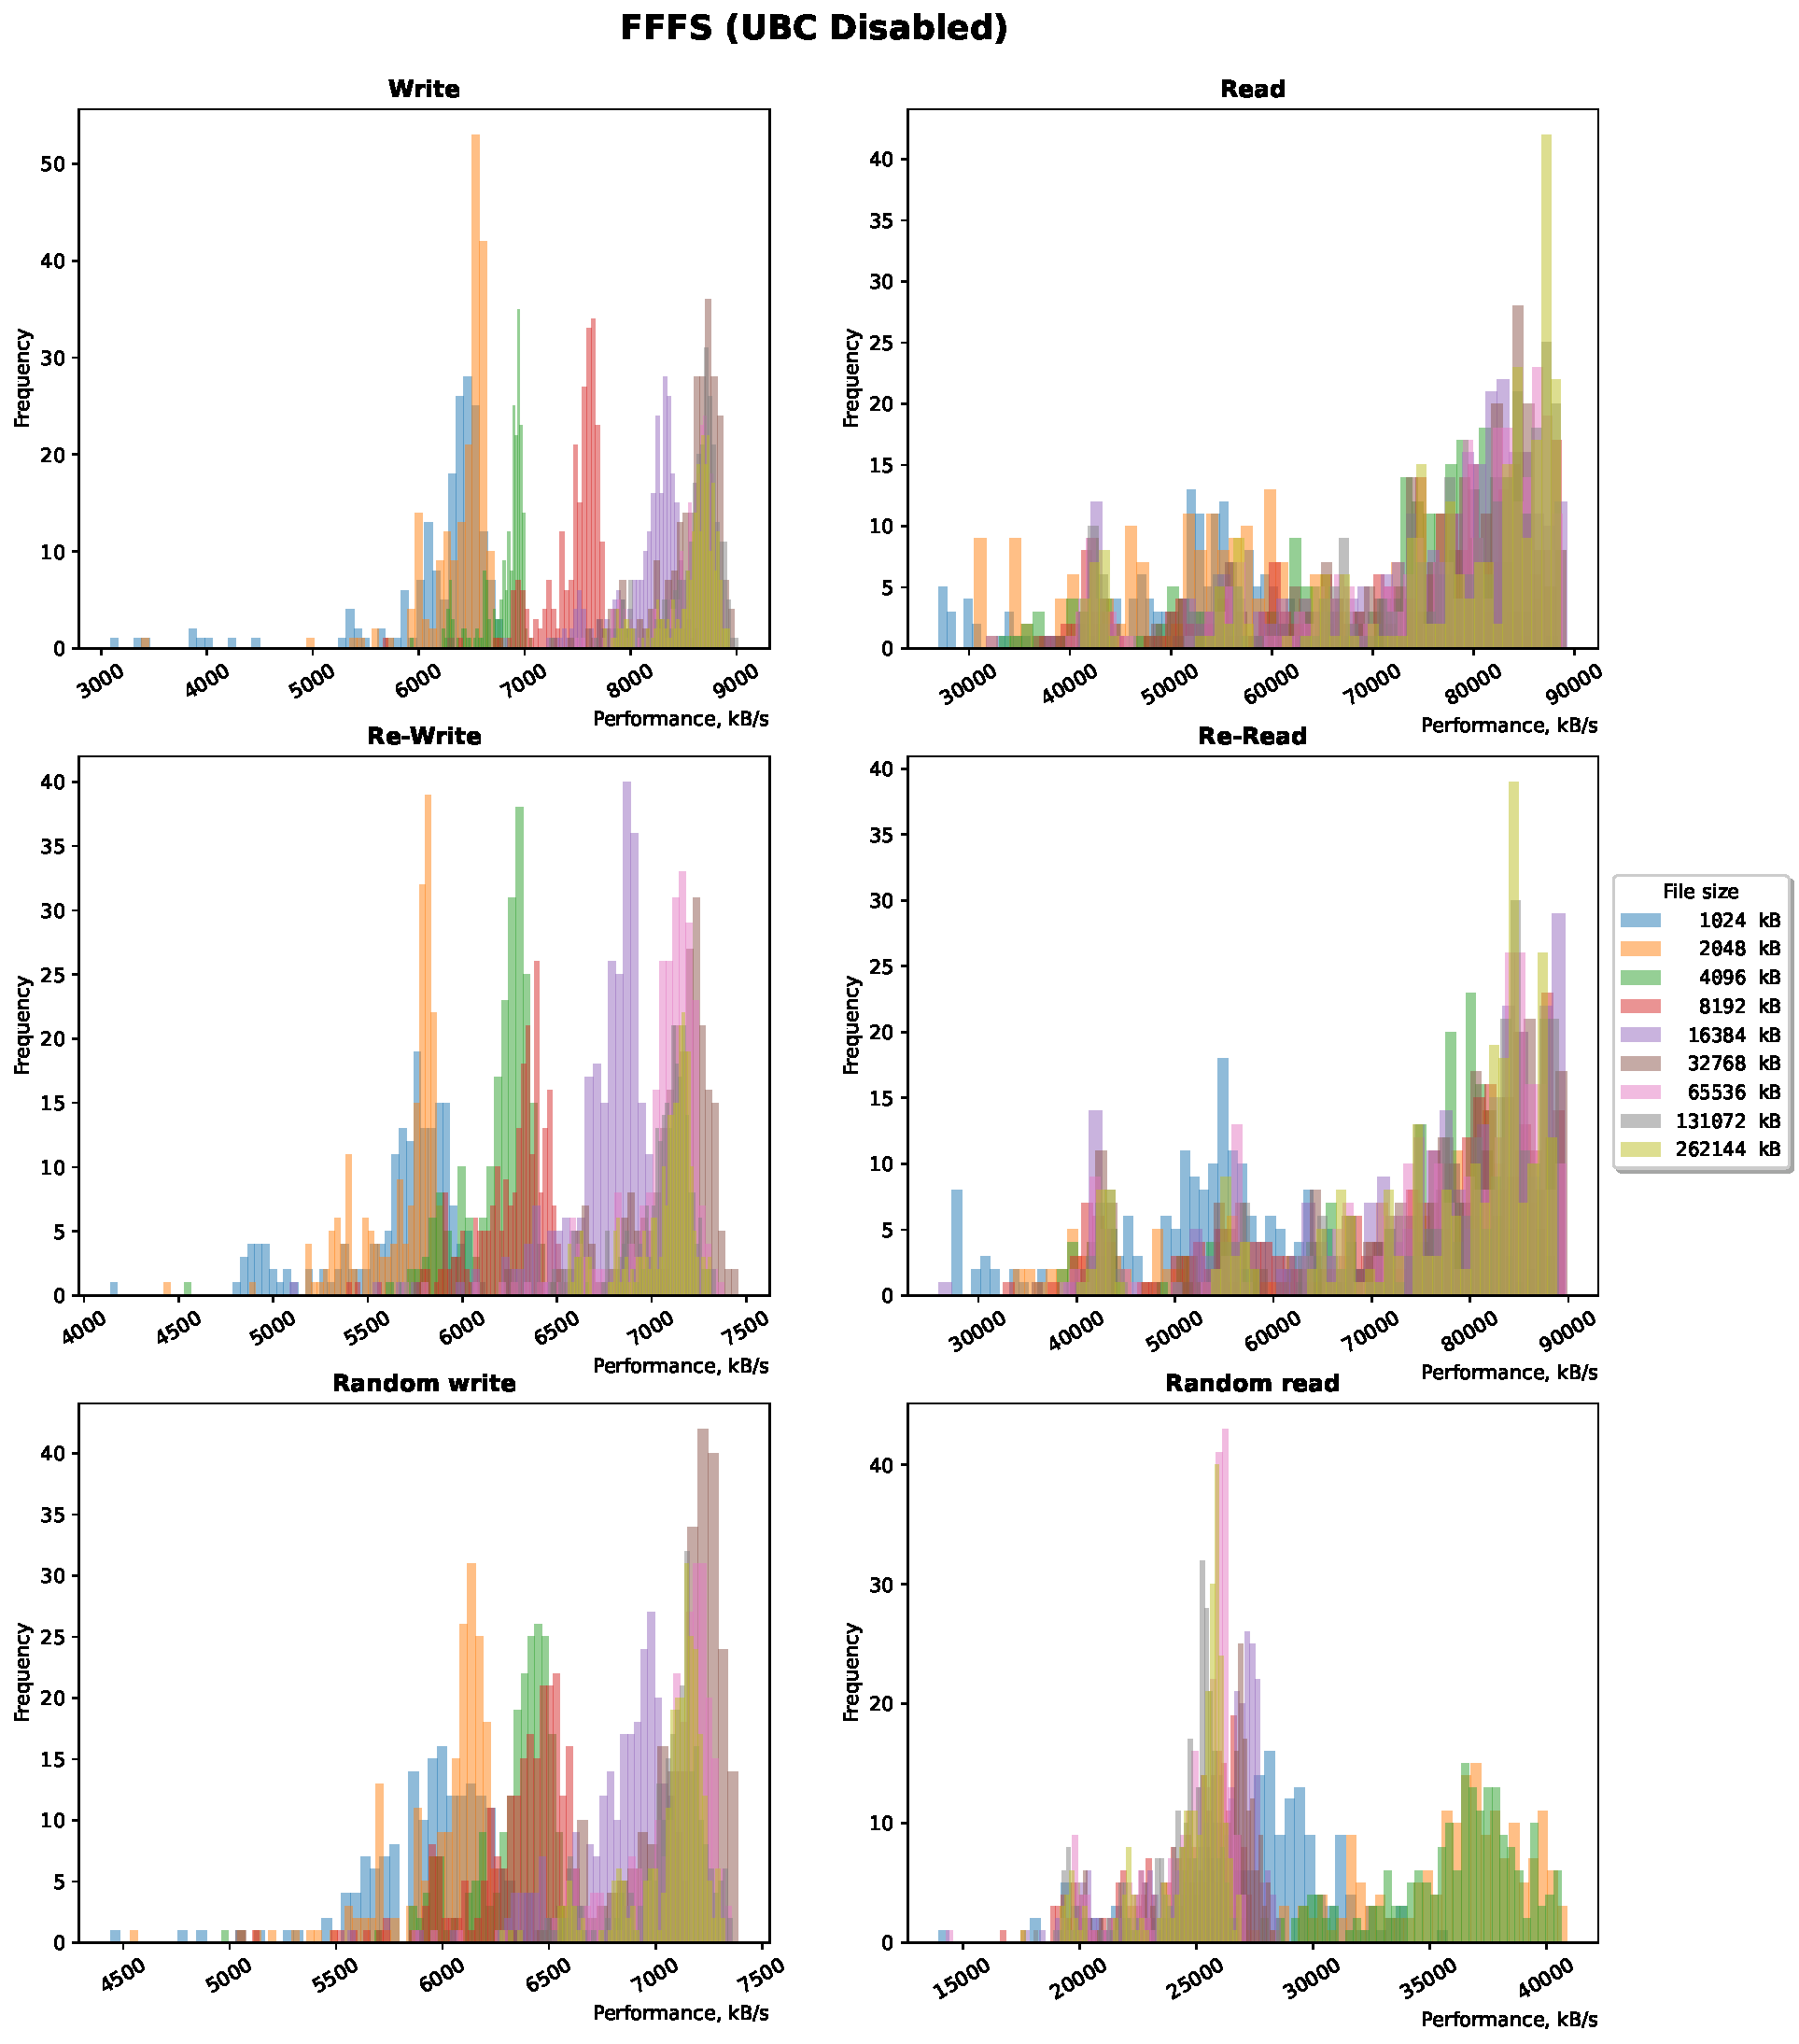
\includegraphics[width=1.0\textwidth]{figures.nosync/benchmarking/FFFS/FFFS-UBC Disabled-hist.pdf}
	\end{center}
	\caption{Performance comparison of different file sizes for FFFS with the UBC disabled}
\end{figure}




\begin{figure}[!htb]
	\label{fig:bench_apfs_with_cache}
	\begin{center}
		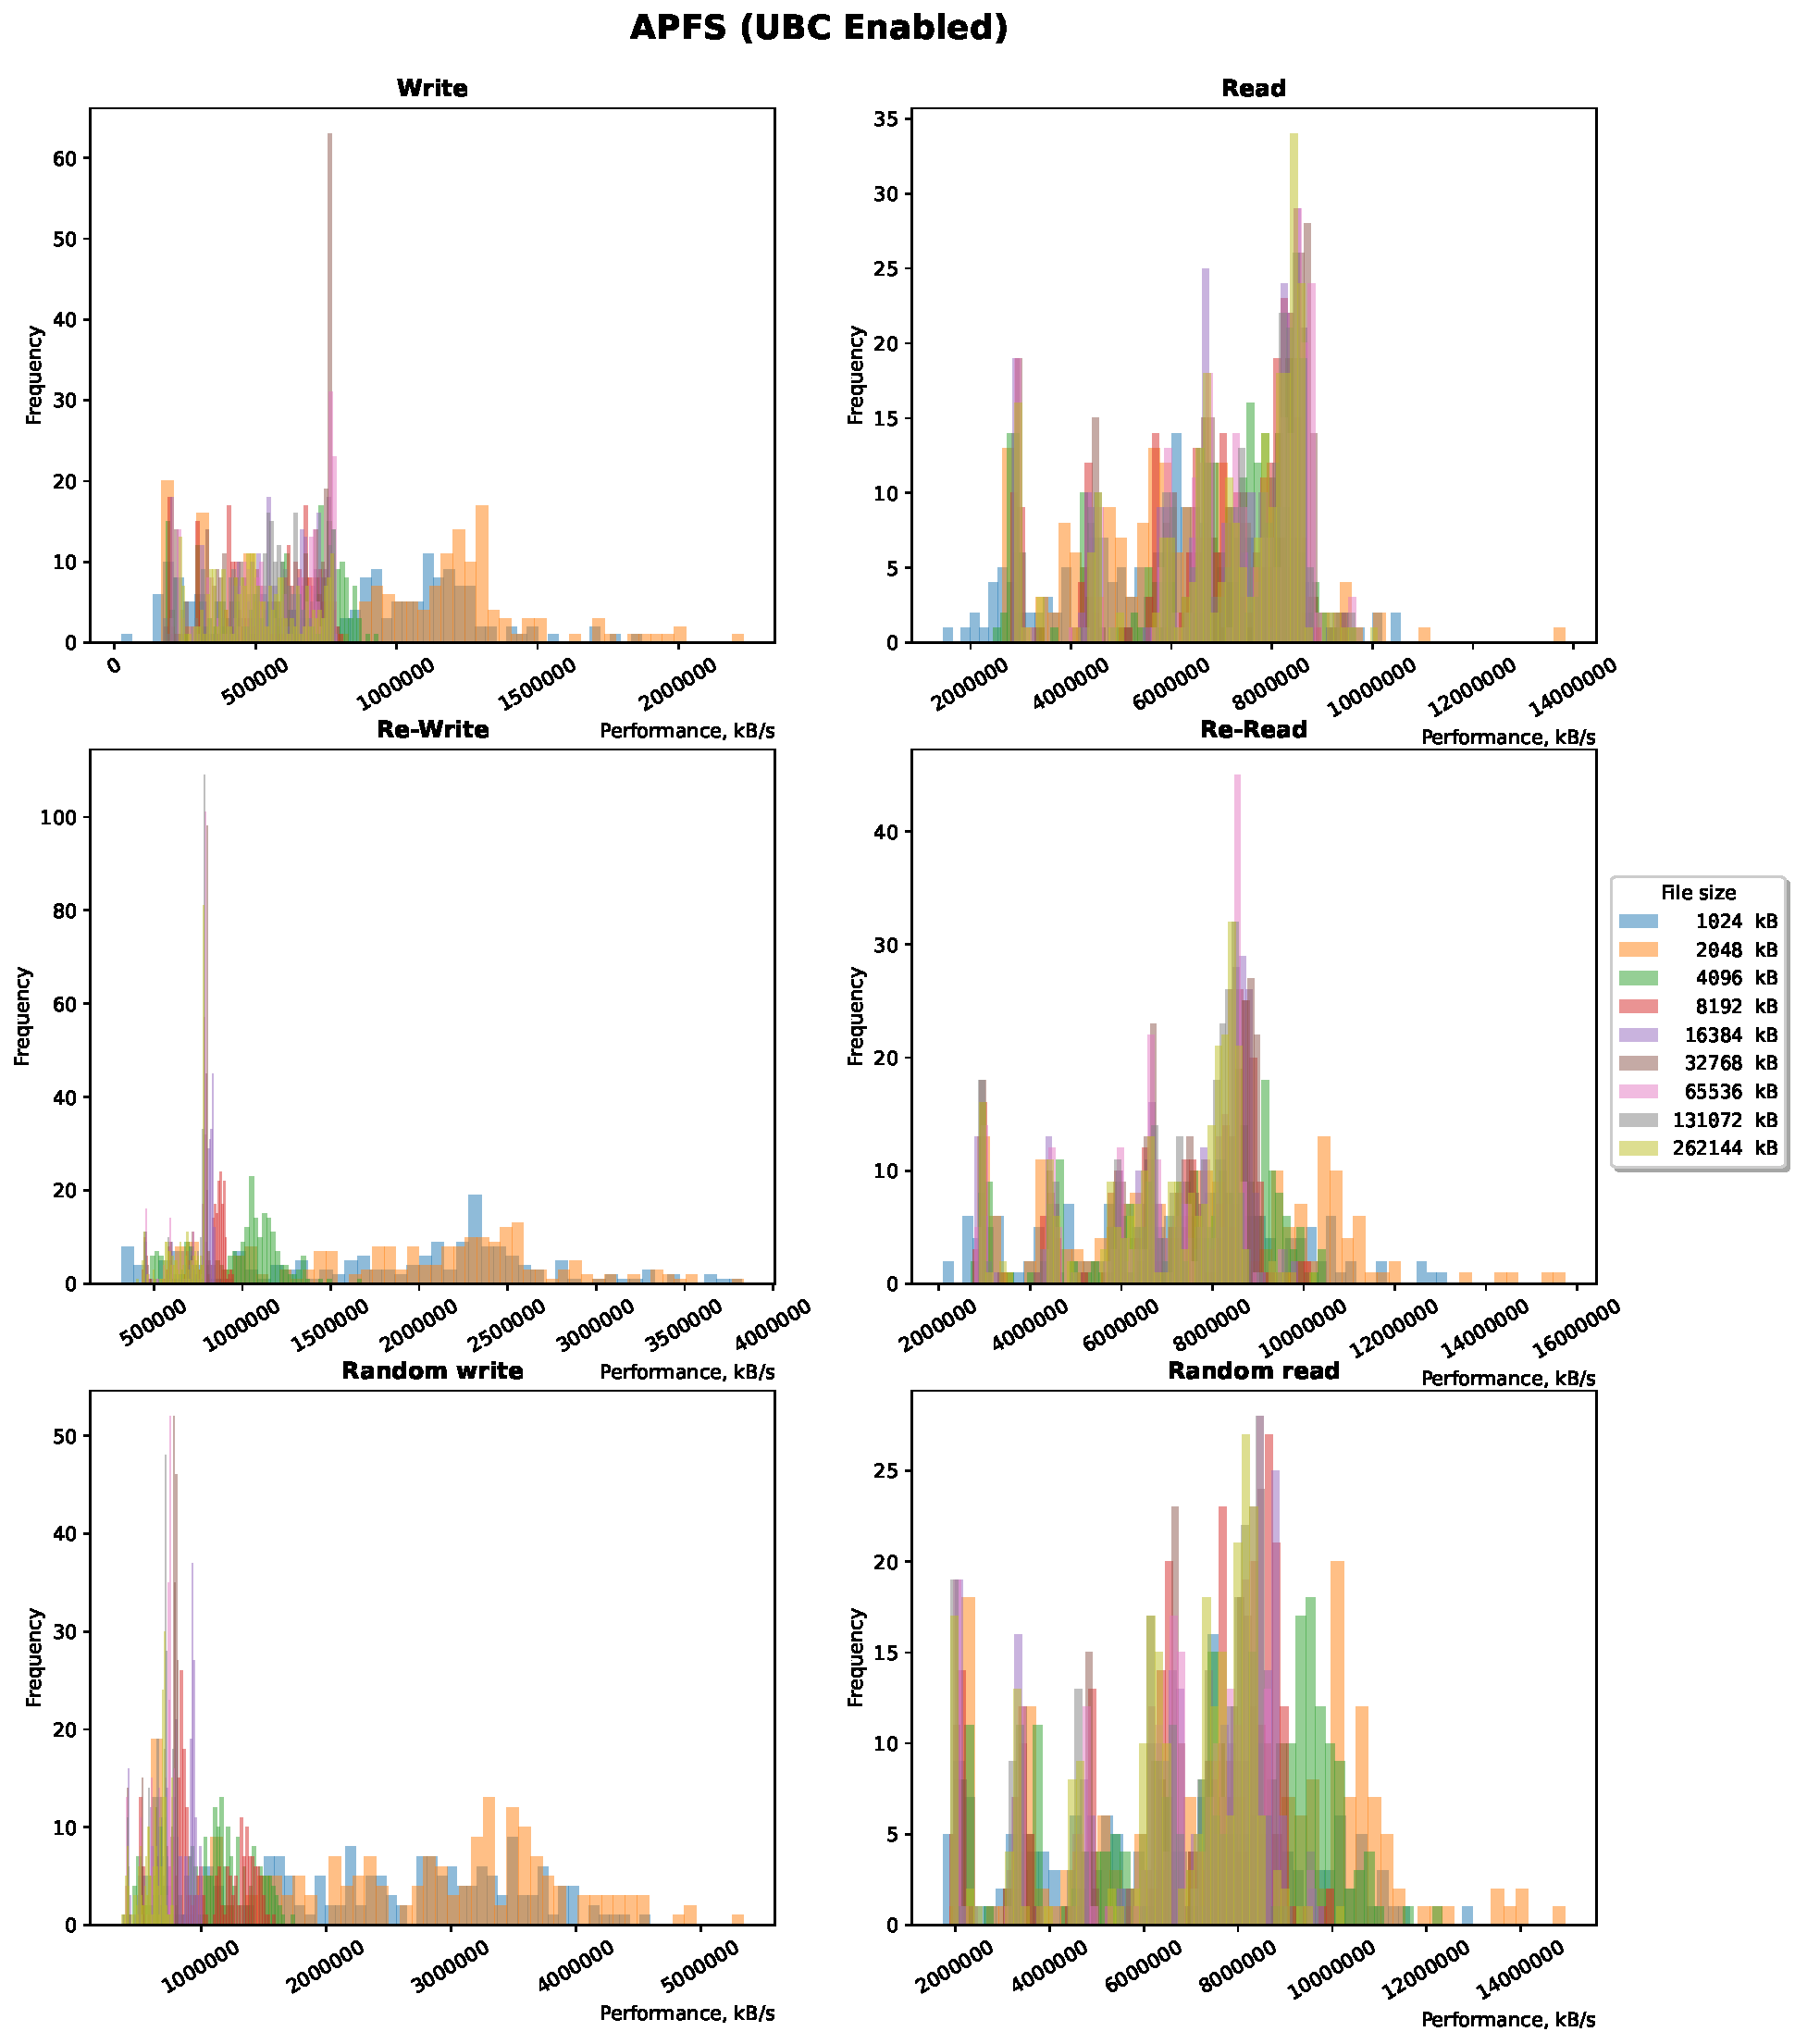
\includegraphics[width=1.0\textwidth]{figures.nosync/benchmarking/APFS/APFS-UBC Enabled-hist.pdf}
	\end{center}
	\caption{Performance comparison of different file sizes for APFS with the UBC enabled}
\end{figure}

\begin{figure}[!htb]
	\label{fig:bench_apfs_without_cache}
	\begin{center}
		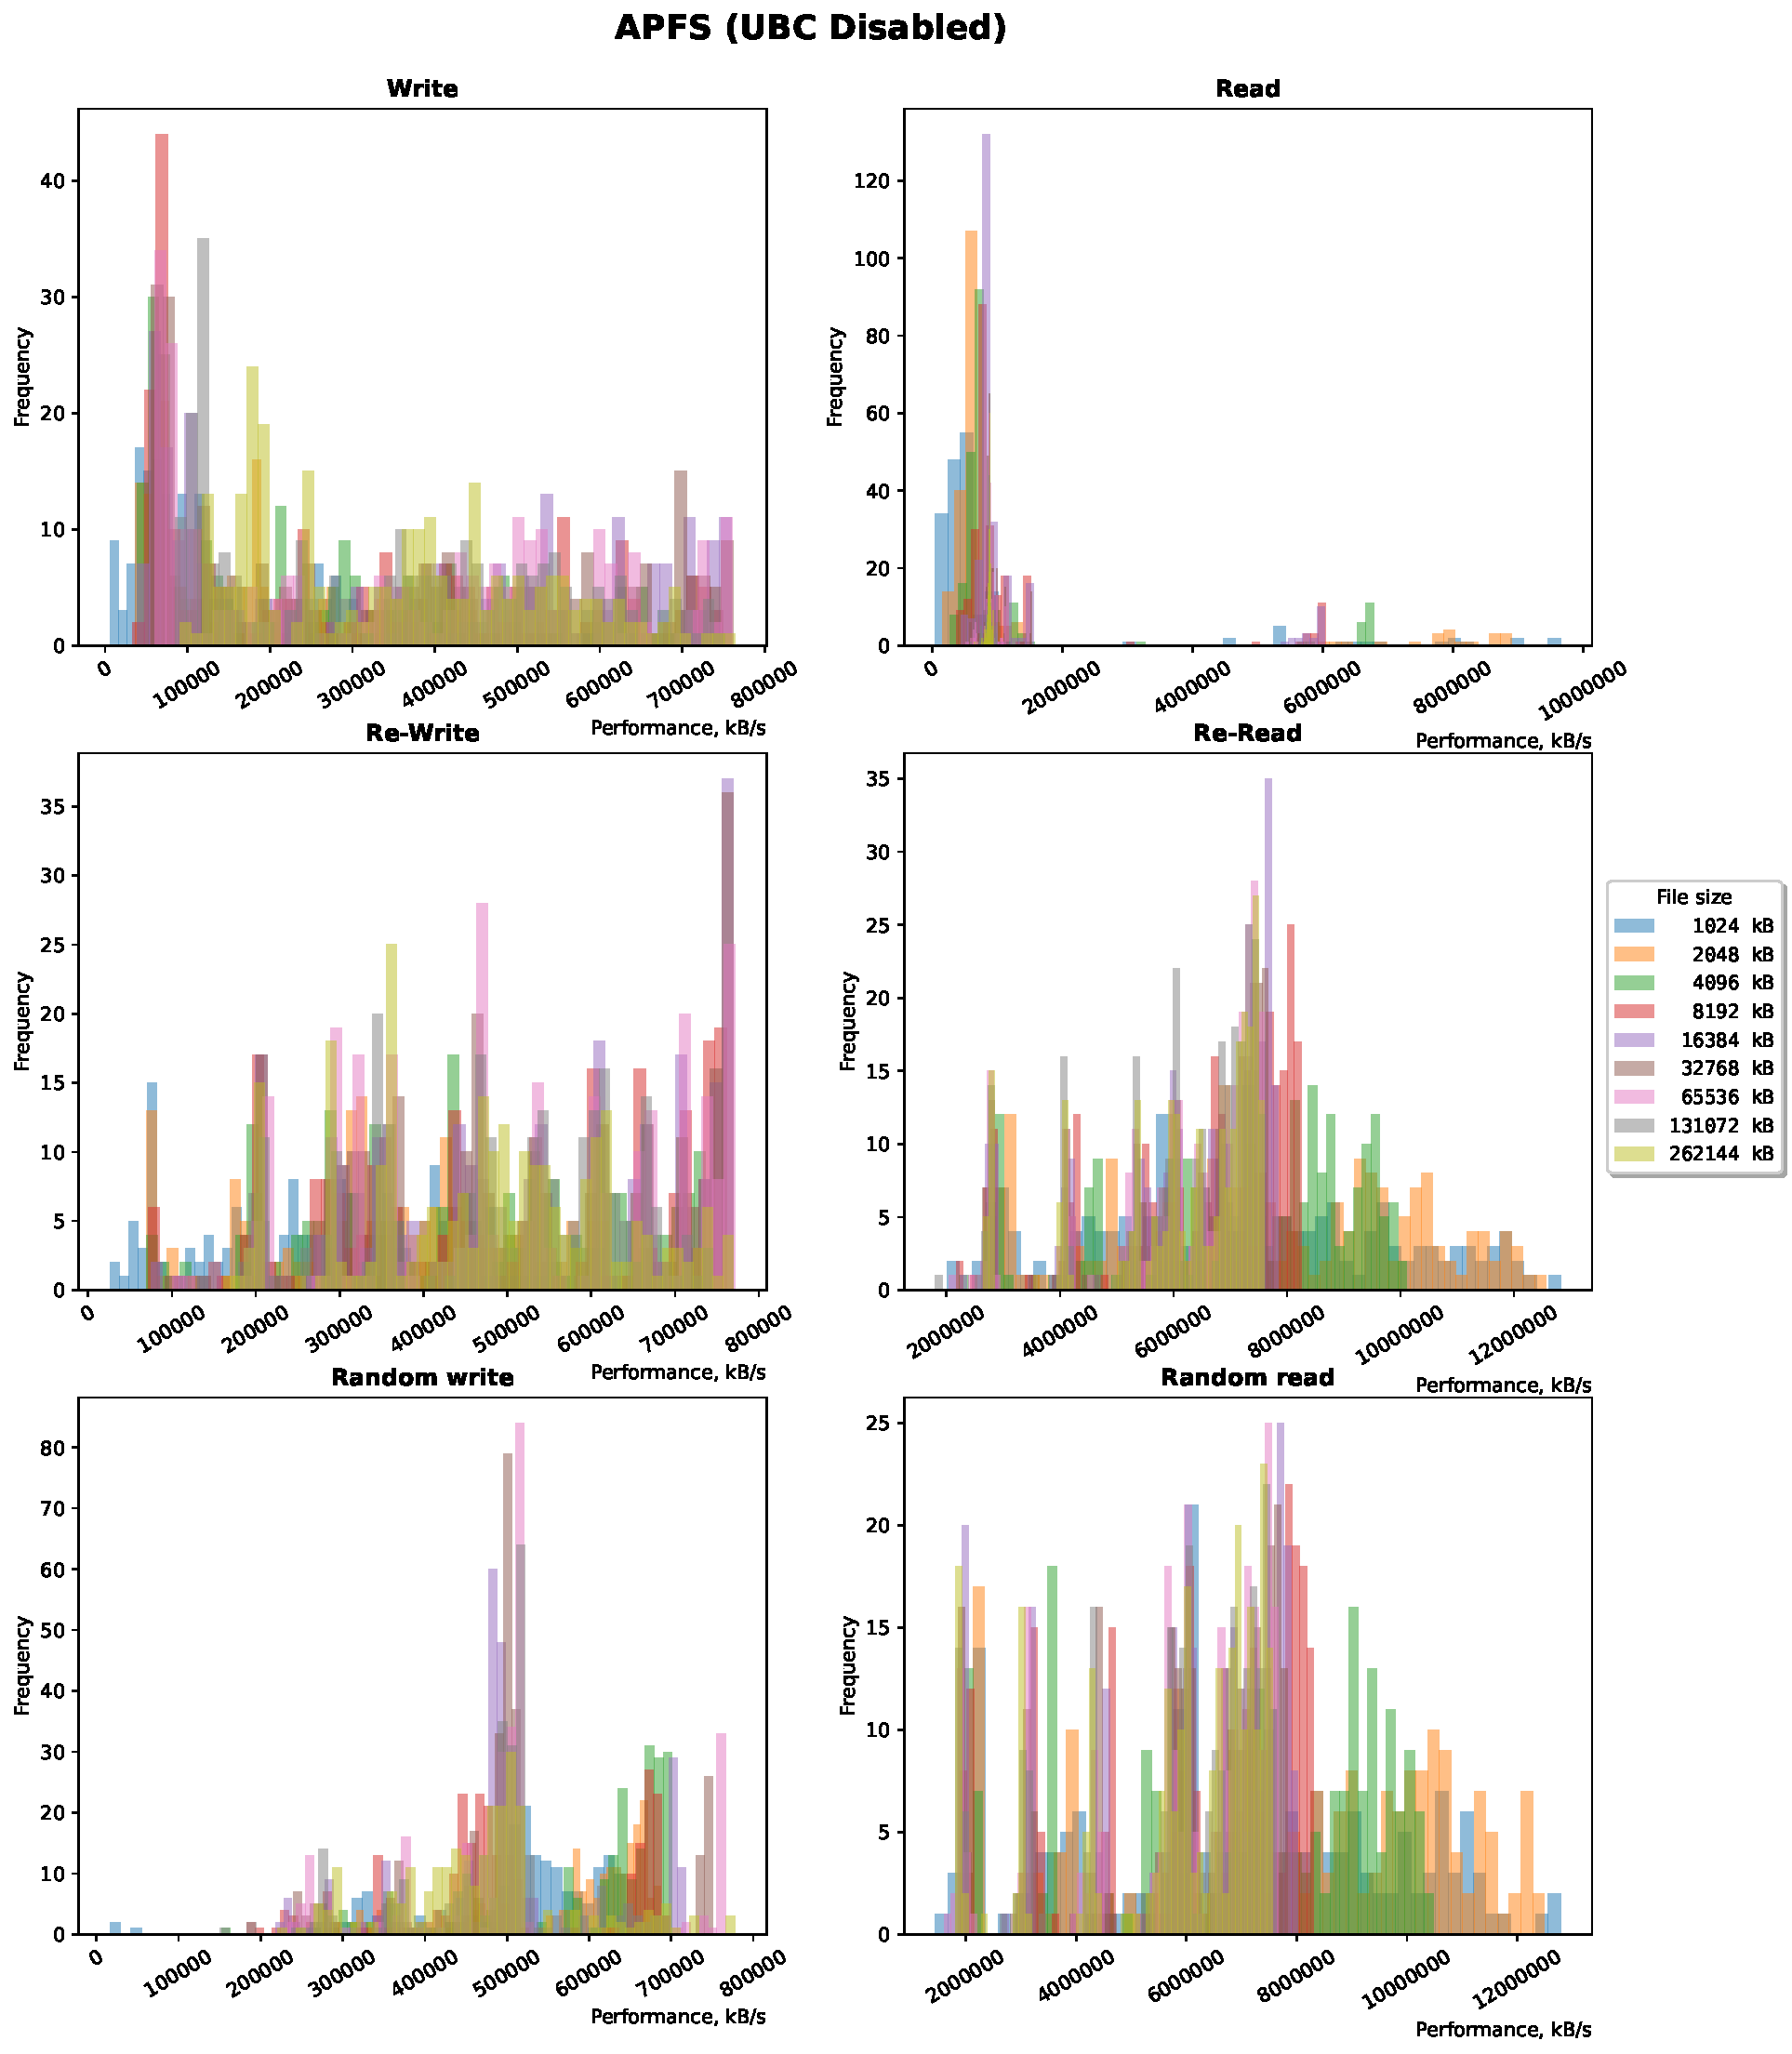
\includegraphics[width=1.0\textwidth]{figures.nosync/benchmarking/APFS/APFS-UBC Disabled-hist.pdf}
	\end{center}
	\caption{Performance comparison of different file sizes for APFS with the UBC disabled}
\end{figure}



% \begin{figure}[!htb]
% 	\label{fig:bench_ffs_read}
% 	\begin{center}
% 		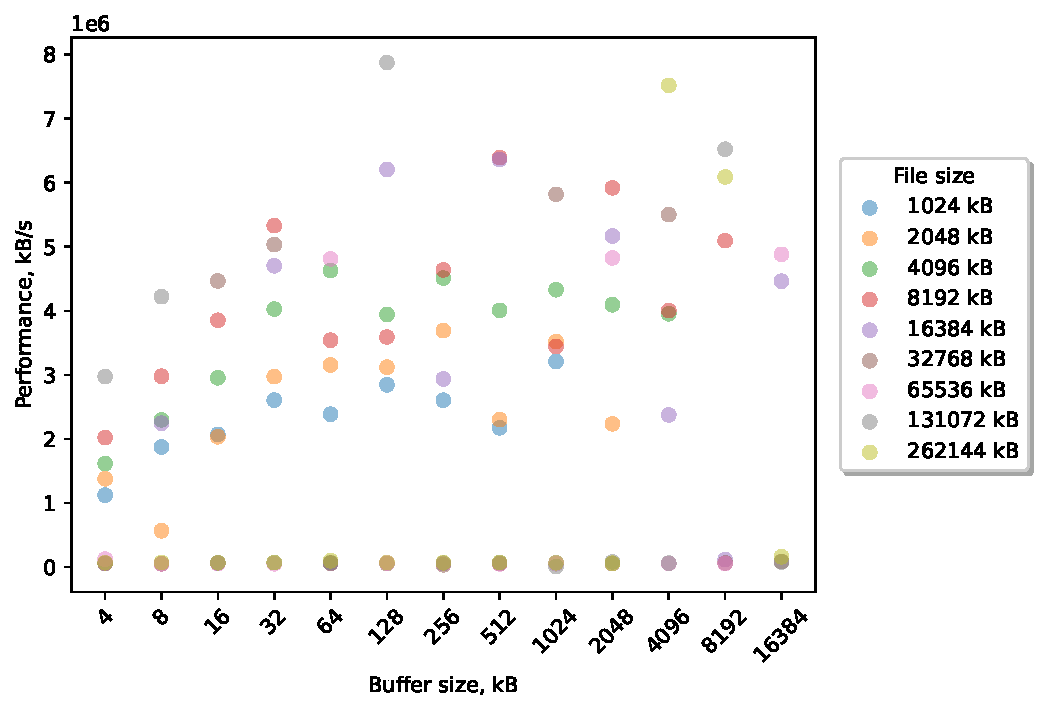
\includegraphics[width=1.0\textwidth]{figures.nosync/benchmarking/old/ffs/Read.pdf}
% 	\end{center}
% 	\caption{IOZone output for FFS Read}
% \end{figure}

% \begin{figure}[!htb]
% 	\label{fig:bench_ffs_write}
% 	\begin{center}
% 		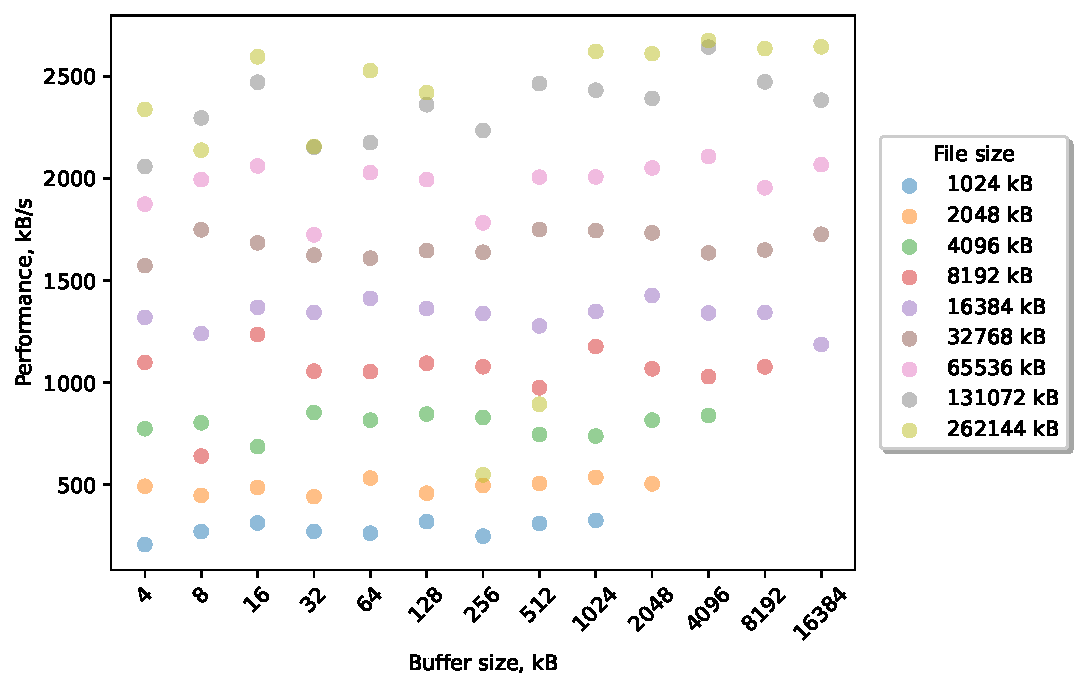
\includegraphics[width=1.0\textwidth]{figures.nosync/benchmarking/old/ffs/Write.pdf}
% 	\end{center}
% 	\caption{IOZone output for FFS Write}
% \end{figure}

% \begin{figure}[!htb]
% 	\label{fig:bench_ffs_re_read}
% 	\begin{center}
% 		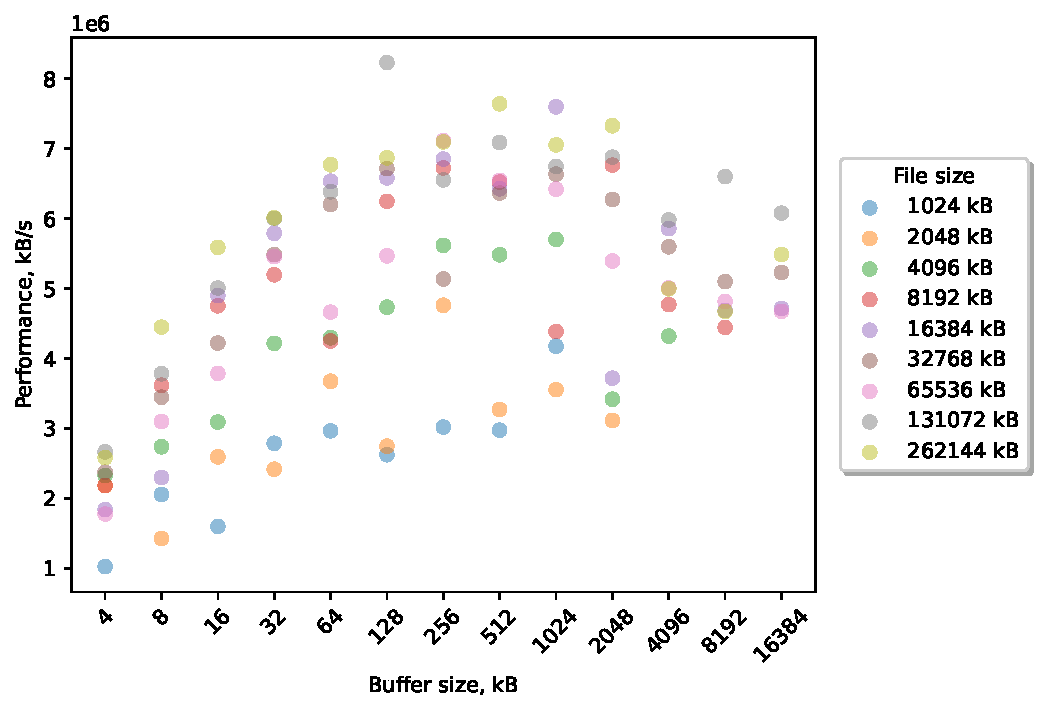
\includegraphics[width=1.0\textwidth]{figures.nosync/benchmarking/old/ffs/Re-Read.pdf}
% 	\end{center}
% 	\caption{IOZone output for FFS \mbox{Re-Read}}
% \end{figure}

% \begin{figure}[!htb]
% 	\label{fig:bench_ffs_re_write}
% 	\begin{center}
% 		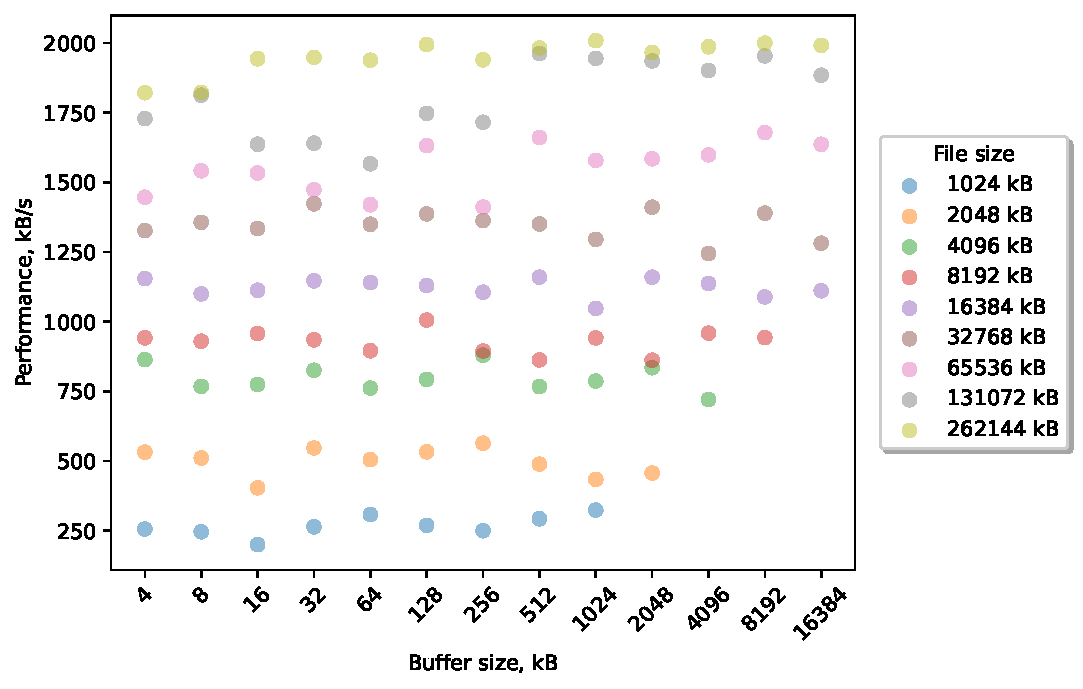
\includegraphics[width=1.0\textwidth]{figures.nosync/benchmarking/old/ffs/Re-Write.pdf}
% 	\end{center}
% 	\caption{IOZone output for FFS \mbox{Re-Write}}
% \end{figure}

% \begin{figure}[!htb]
% 	\label{fig:bench_ffs_rnd_read}
% 	\begin{center}
% 		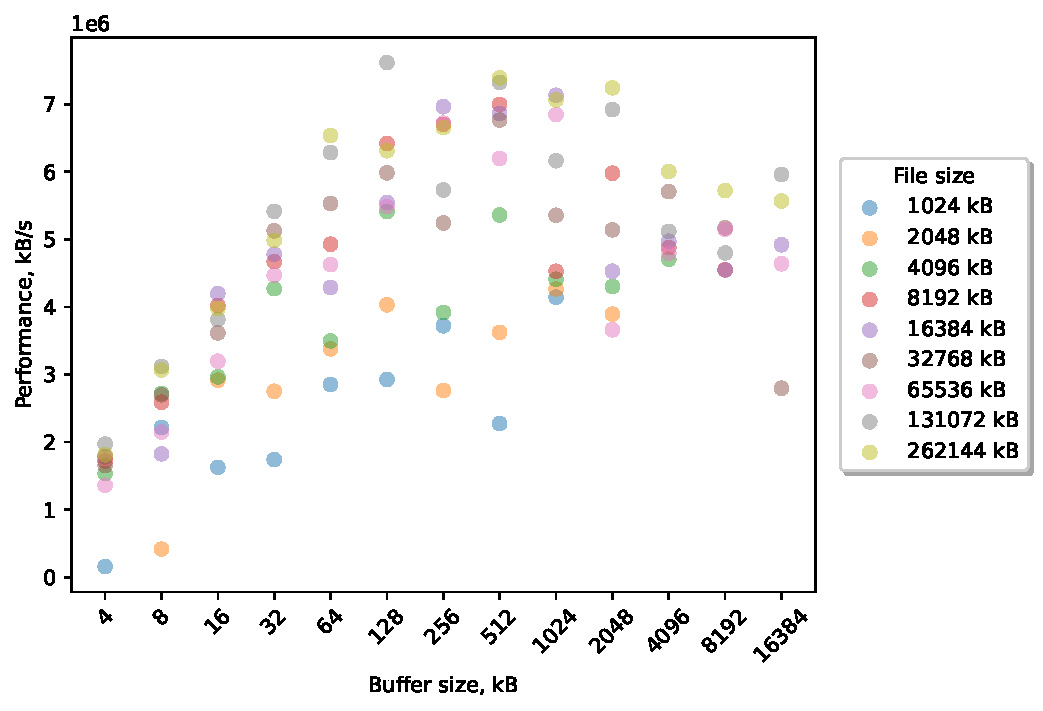
\includegraphics[width=1.0\textwidth]{figures.nosync/benchmarking/old/ffs/Random read.pdf}
% 	\end{center}
% 	\caption{IOZone output for FFS Random read}
% \end{figure}

% \begin{figure}[!htb]
% 	\label{fig:bench_ffs_rnd_write}
% 	\begin{center}
% 		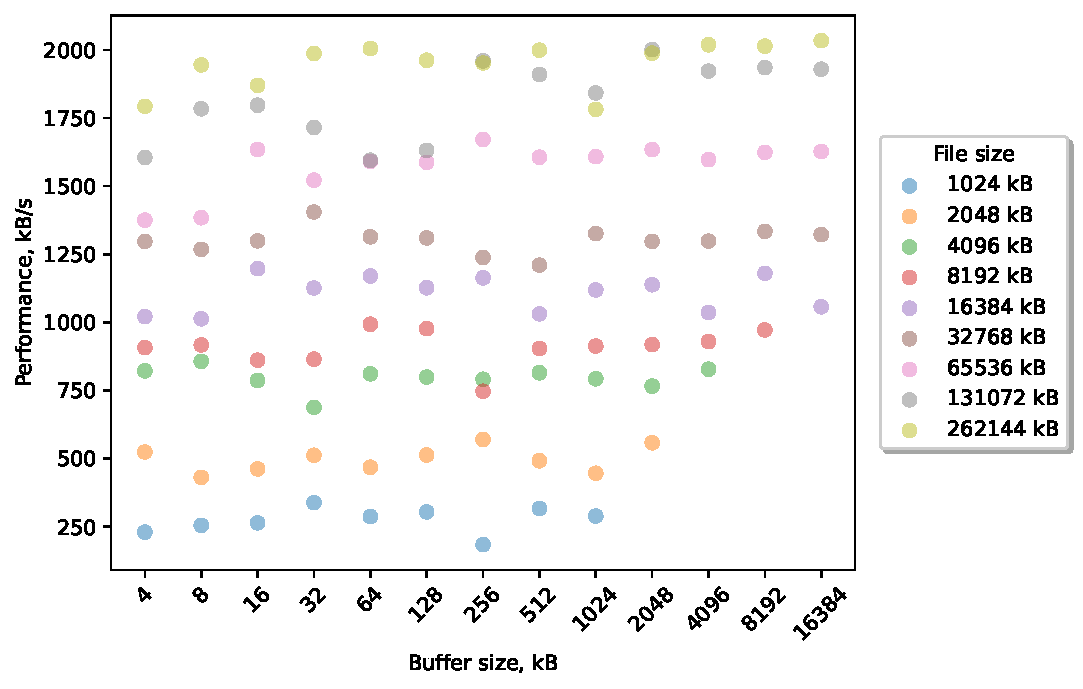
\includegraphics[width=1.0\textwidth]{figures.nosync/benchmarking/old/ffs/Random write.pdf}
% 	\end{center}
% 	\caption{IOZone output for FFS Random write}
% \end{figure}

% \begin{figure}[!htb]
% 	\label{fig:bench_fffs_read}
% 	\begin{center}
% 		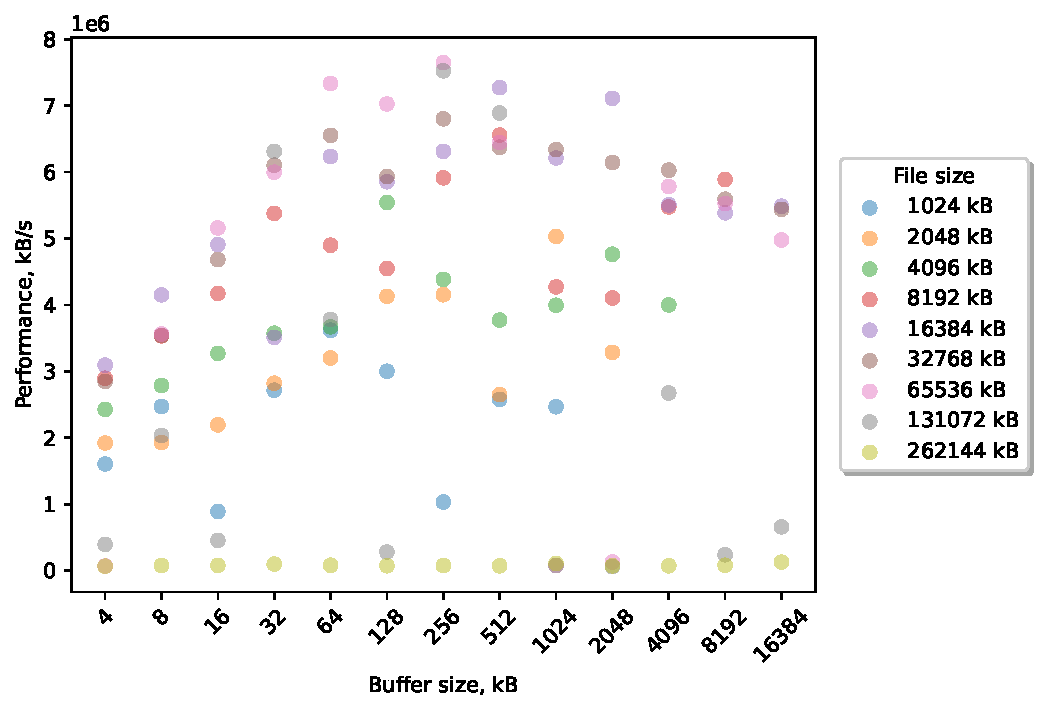
\includegraphics[width=1.0\textwidth]{figures.nosync/benchmarking/old/fejk-ffs/Read.pdf}
% 	\end{center}
% 	\caption{IOZone output for Fejk FFS Read}
% \end{figure}

% \begin{figure}[!htb]
% 	\label{fig:bench_fffs_write}
% 	\begin{center}
% 		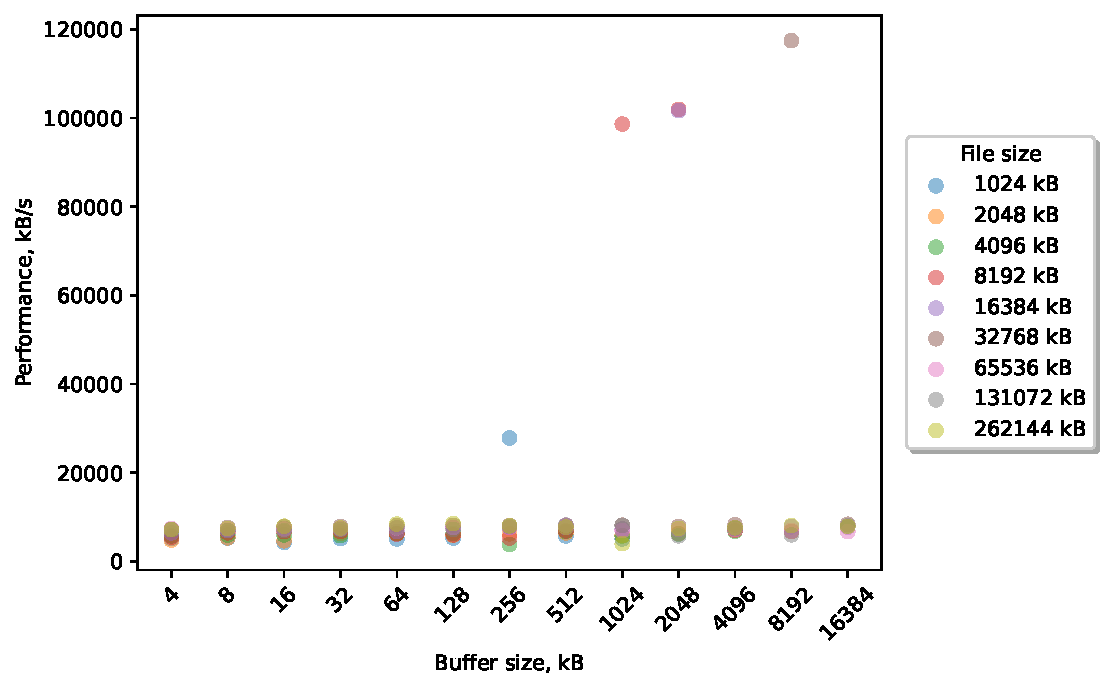
\includegraphics[width=1.0\textwidth]{figures.nosync/benchmarking/old/fejk-ffs/Write.pdf}
% 	\end{center}
% 	\caption{IOZone output for Fejk FFS Write}
% \end{figure}

% \begin{figure}[!htb]
% 	\label{fig:bench_fffs_re_read}
% 	\begin{center}
% 		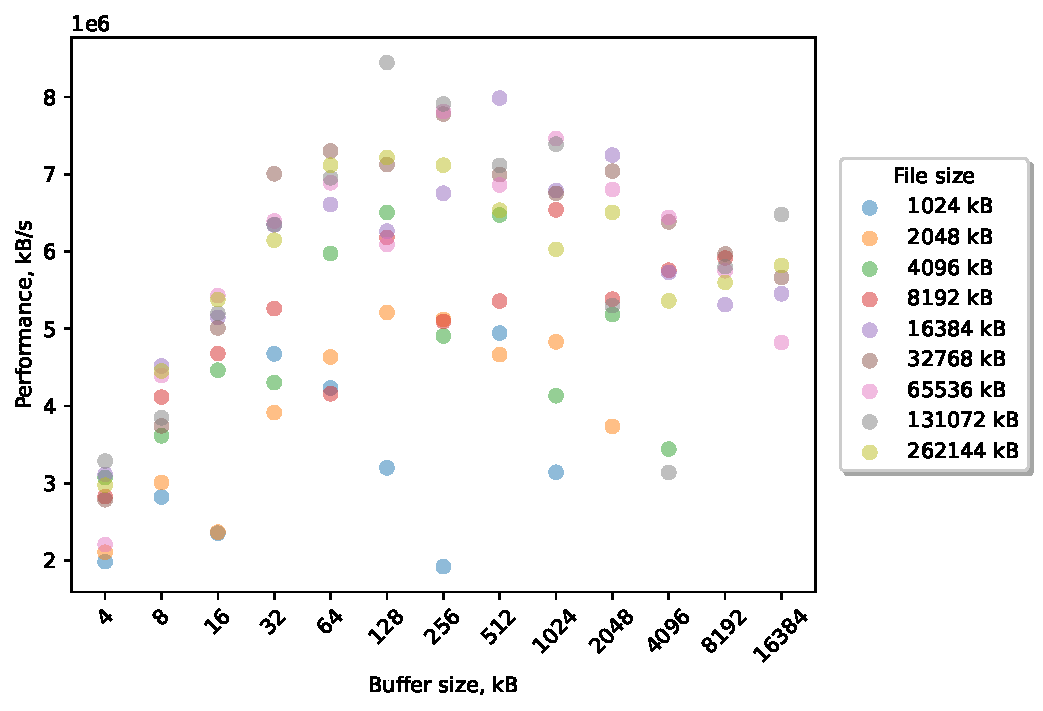
\includegraphics[width=1.0\textwidth]{figures.nosync/benchmarking/old/fejk-ffs/Re-Read.pdf}
% 	\end{center}
% 	\caption{IOZone output for Fejk FFS \mbox{Re-Read}}
% \end{figure}

% \begin{figure}[!htb]
% 	\label{fig:bench_fffs_re_write}
% 	\begin{center}
% 		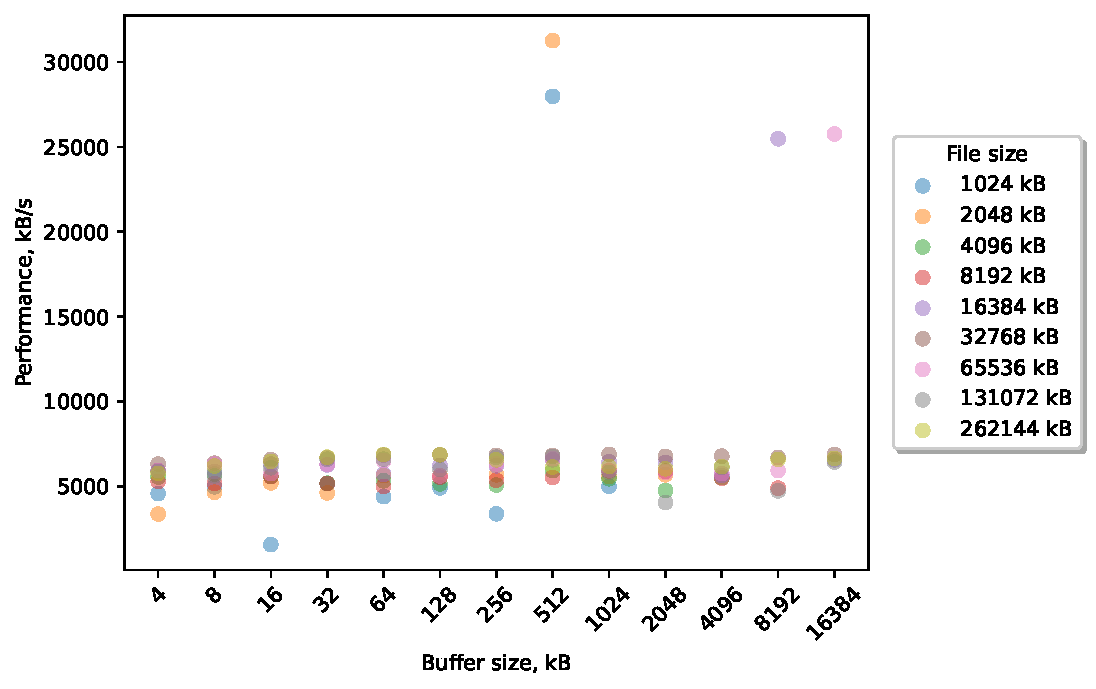
\includegraphics[width=1.0\textwidth]{figures.nosync/benchmarking/old/fejk-ffs/Re-Write.pdf}
% 	\end{center}
% 	\caption{IOZone output for Fejk FFS \mbox{Re-Write}}
% \end{figure}

% \begin{figure}[!htb]
% 	\label{fig:bench_fffs_rnd_read}
% 	\begin{center}
% 		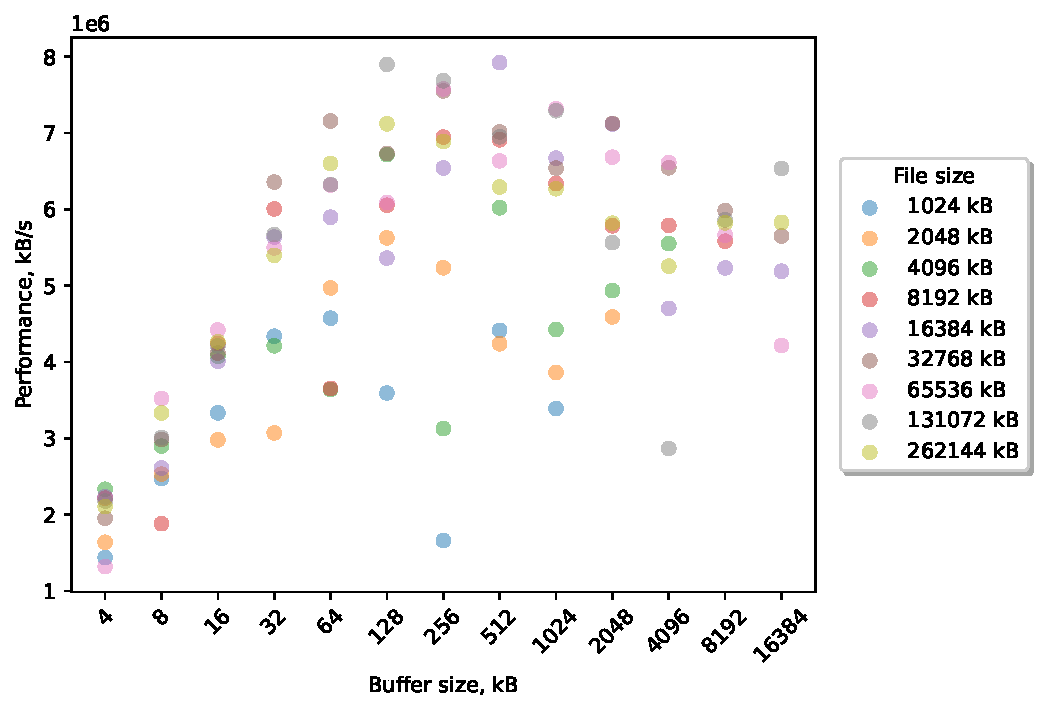
\includegraphics[width=1.0\textwidth]{figures.nosync/benchmarking/old/fejk-ffs/Random read.pdf}
% 	\end{center}
% 	\caption{IOZone output for Fejk FFS Random read}
% \end{figure}

% \begin{figure}[!htb]
% 	\label{fig:bench_fffs_rnd_write}
% 	\begin{center}
% 		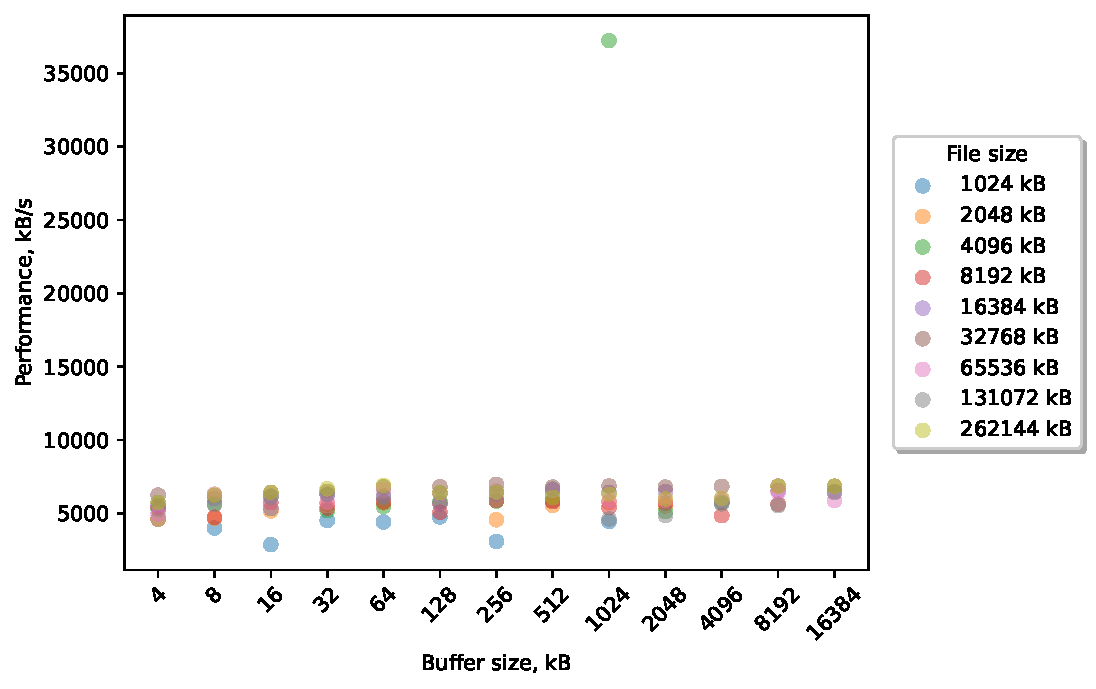
\includegraphics[width=1.0\textwidth]{figures.nosync/benchmarking/old/fejk-ffs/Random write.pdf}
% 	\end{center}
% 	\caption{IOZone output for Fejk FFS Random write}
% \end{figure}

% \begin{figure}[!htb]
% 	\label{fig:bench_gcsf_read}
% 	\begin{center}
% 		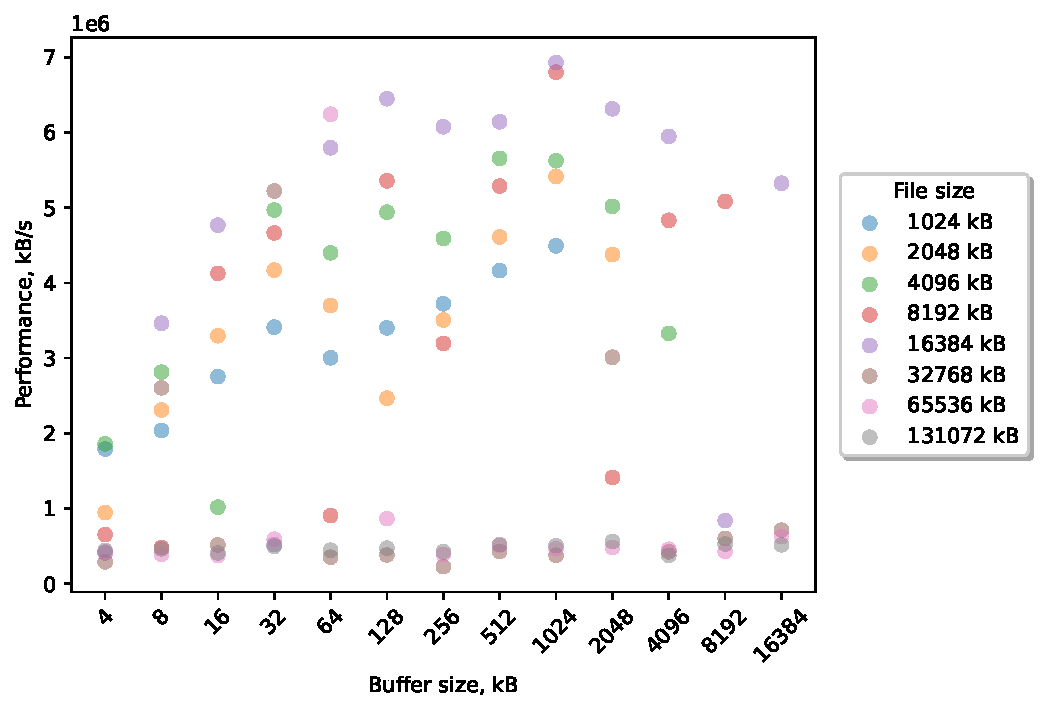
\includegraphics[width=1.0\textwidth]{figures.nosync/benchmarking/old/gcsf/Read.pdf}
% 	\end{center}
% 	\caption{IOZone output for GCSF Read}
% \end{figure}

% \begin{figure}[!htb]
% 	\label{fig:bench_gcsf_write}
% 	\begin{center}
% 		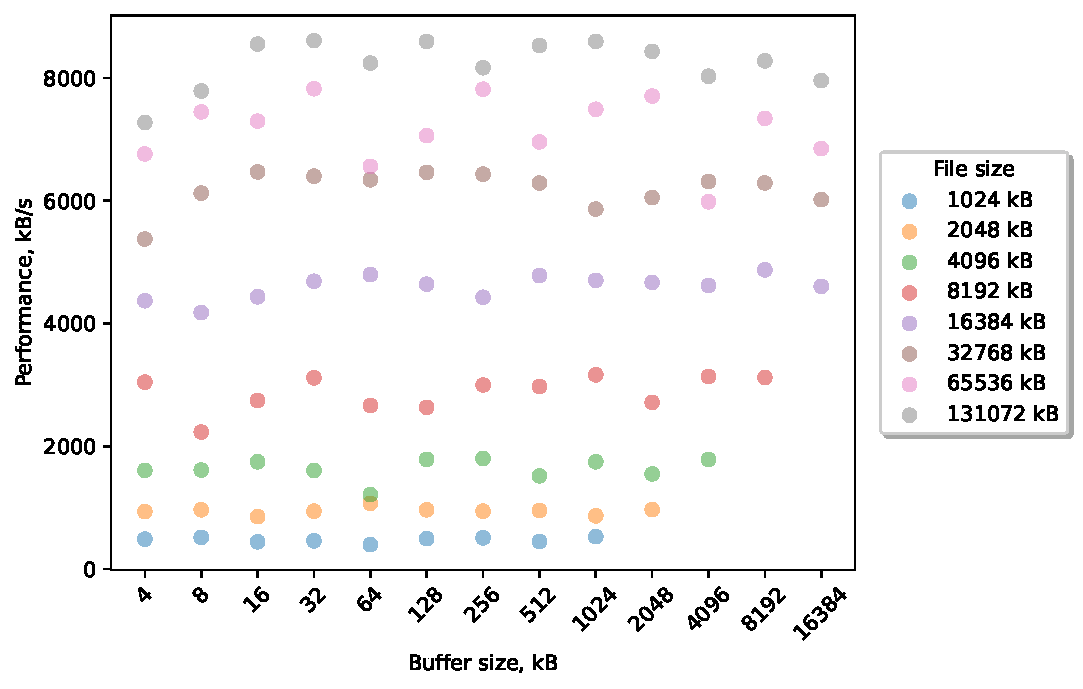
\includegraphics[width=1.0\textwidth]{figures.nosync/benchmarking/old/gcsf/Write.pdf}
% 	\end{center}
% 	\caption{IOZone output for GCSF Write}
% \end{figure}

% \begin{figure}[!htb]
% 	\label{fig:bench_gcsf_re_read}
% 	\begin{center}
% 		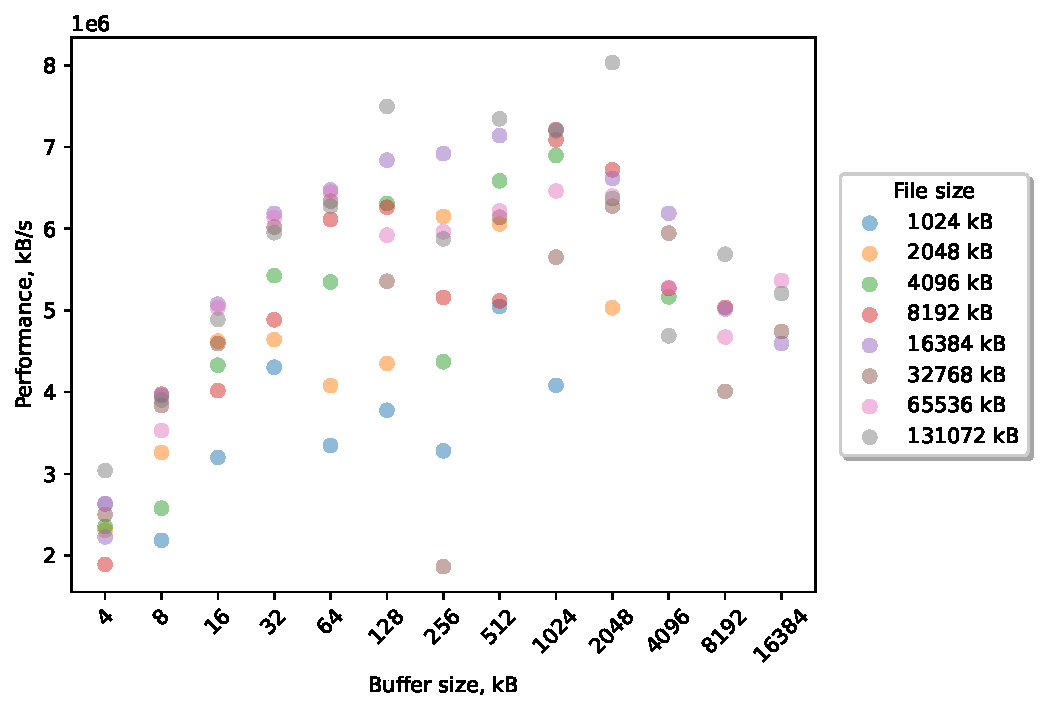
\includegraphics[width=1.0\textwidth]{figures.nosync/benchmarking/old/gcsf/Re-Read.pdf}
% 	\end{center}
% 	\caption{IOZone output for GCSF \mbox{Re-Read}}
% \end{figure}

% \begin{figure}[!htb]
% 	\label{fig:bench_gcsf_re_write}
% 	\begin{center}
% 		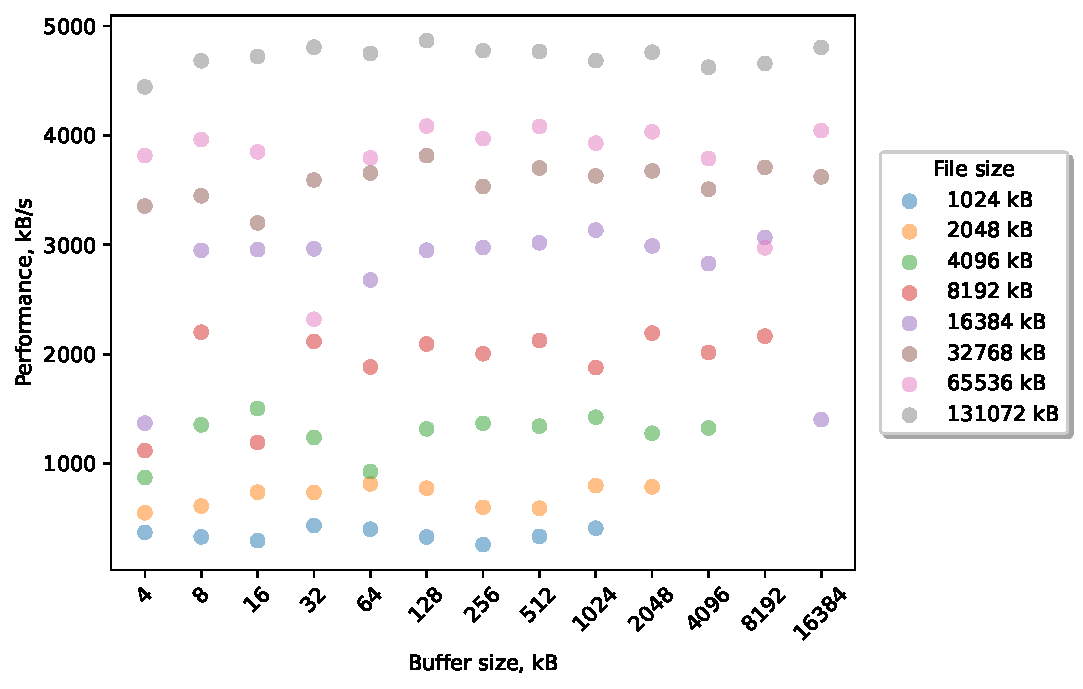
\includegraphics[width=1.0\textwidth]{figures.nosync/benchmarking/old/gcsf/Re-Write.pdf}
% 	\end{center}
% 	\caption{IOZone output for GCSF \mbox{Re-Write}}
% \end{figure}

% \begin{figure}[!htb]
% 	\label{fig:bench_gcsf_rnd_read}
% 	\begin{center}
% 		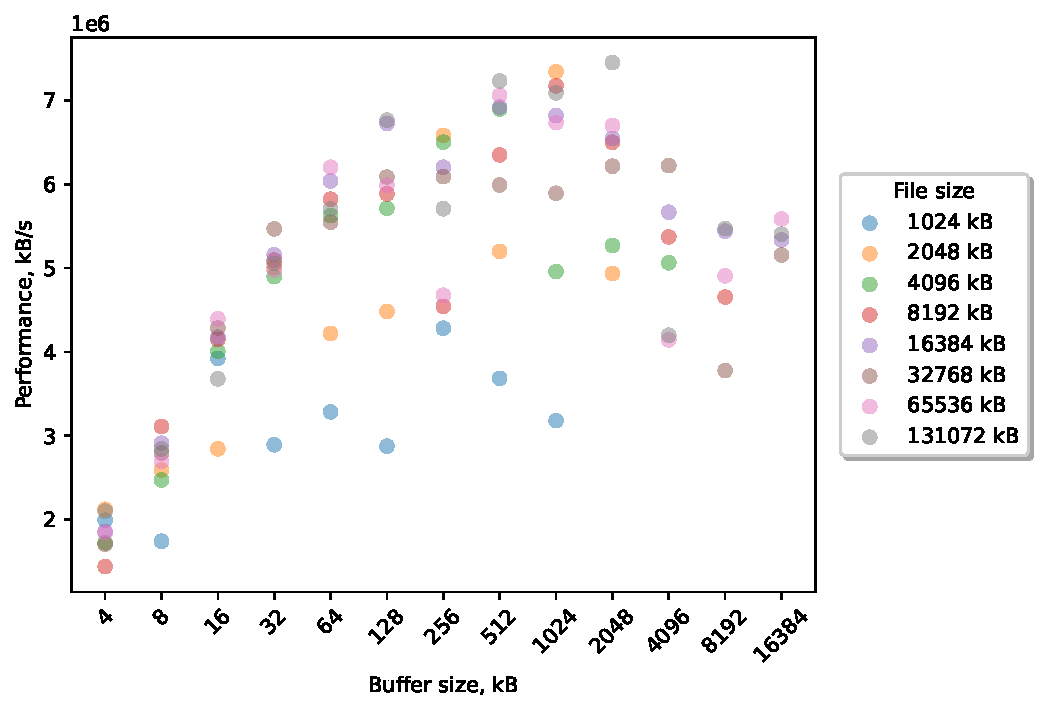
\includegraphics[width=1.0\textwidth]{figures.nosync/benchmarking/old/gcsf/Random read.pdf}
% 	\end{center}
% 	\caption{IOZone output for GCSF Random read}
% \end{figure}

% \begin{figure}[!htb]
% 	\label{fig:bench_gcsf_rnd_write}
% 	\begin{center}
% 		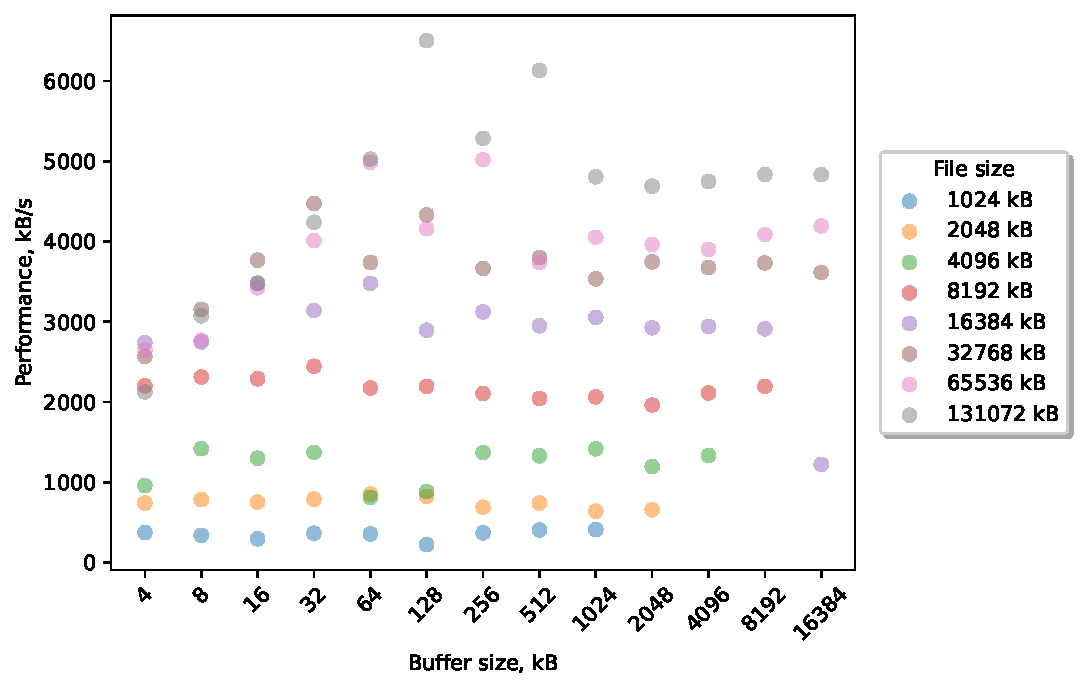
\includegraphics[width=1.0\textwidth]{figures.nosync/benchmarking/old/gcsf/Random write.pdf}
% 	\end{center}
% 	\caption{IOZone output for GCSF Random write}
% \end{figure}

% \begin{figure}[!htb]
% 	\label{fig:bench_apfs_read}
% 	\begin{center}
% 		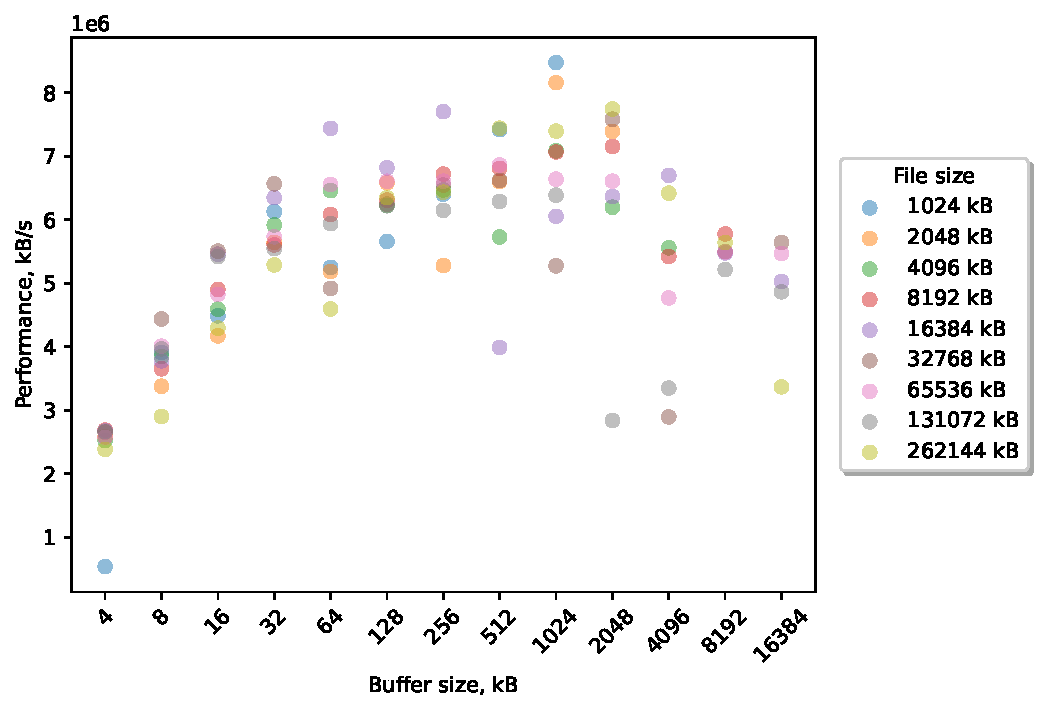
\includegraphics[width=1.0\textwidth]{figures.nosync/benchmarking/old/local/Read.pdf}
% 	\end{center}
% 	\caption{IOZone output for \gls{APFS} Read}
% \end{figure}

% \begin{figure}[!htb]
% 	\label{fig:bench_apfs_write}
% 	\begin{center}
% 		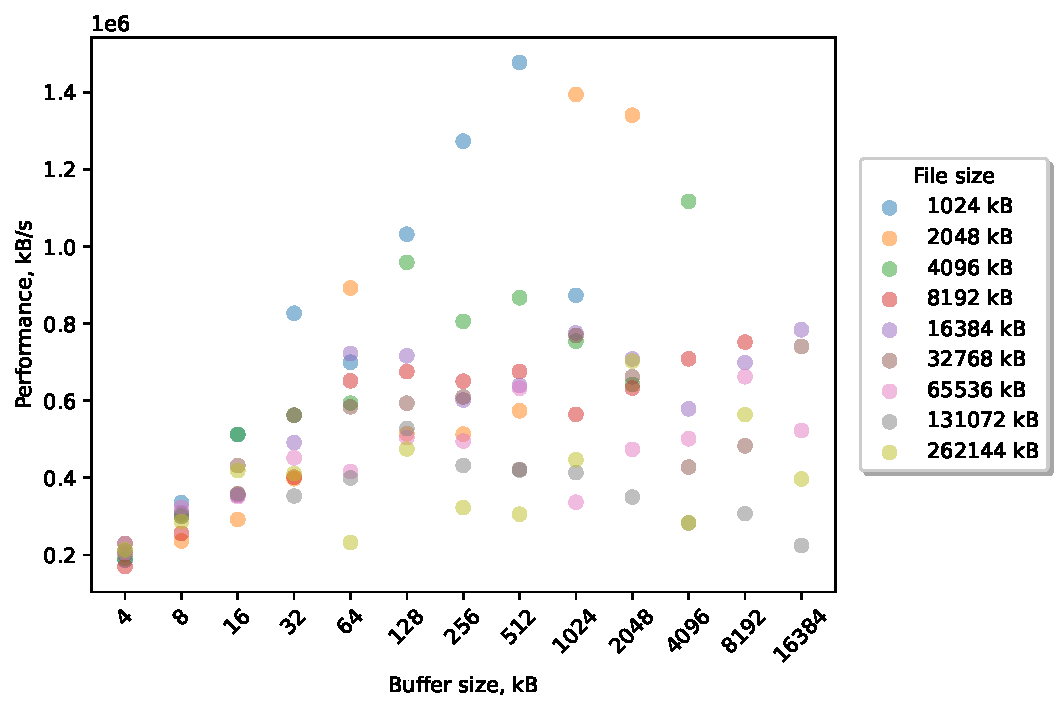
\includegraphics[width=1.0\textwidth]{figures.nosync/benchmarking/old/local/Write.pdf}
% 	\end{center}
% 	\caption{IOZone output for \gls{APFS} Write}
% \end{figure}

% \begin{figure}[!htb]
% 	\label{fig:bench_apfs_re_read}
% 	\begin{center}
% 		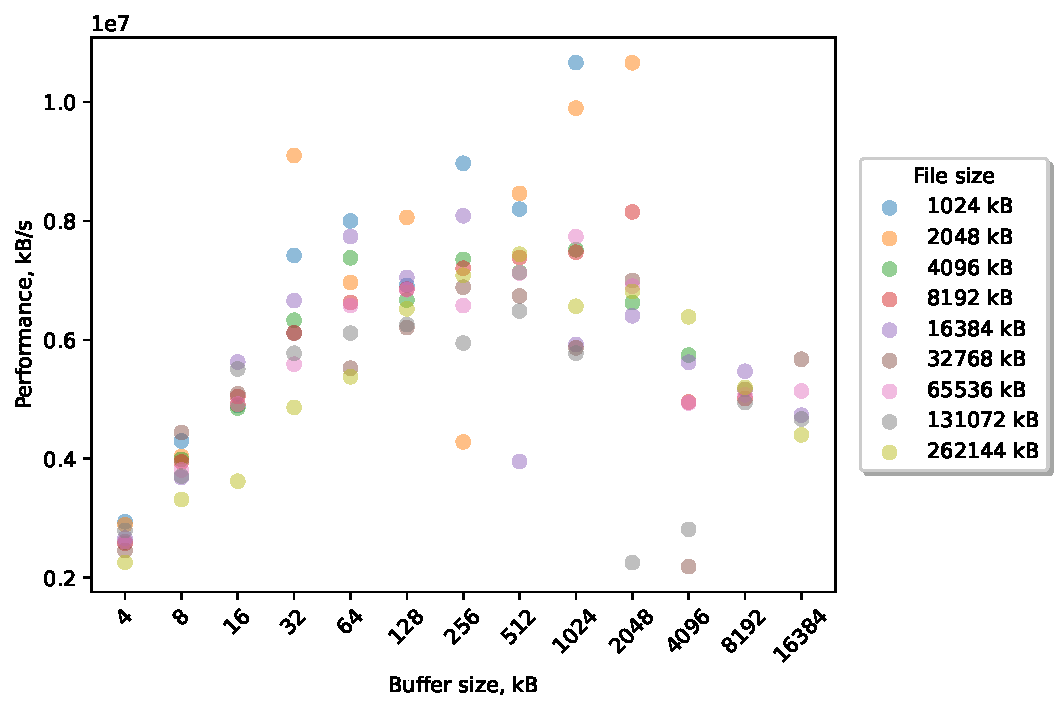
\includegraphics[width=1.0\textwidth]{figures.nosync/benchmarking/old/local/Re-Read.pdf}
% 	\end{center}
% 	\caption{IOZone output for \gls{APFS} \mbox{Re-Read}}
% \end{figure}

% \begin{figure}[!htb]
% 	\label{fig:bench_apfs_re_write}
% 	\begin{center}
% 		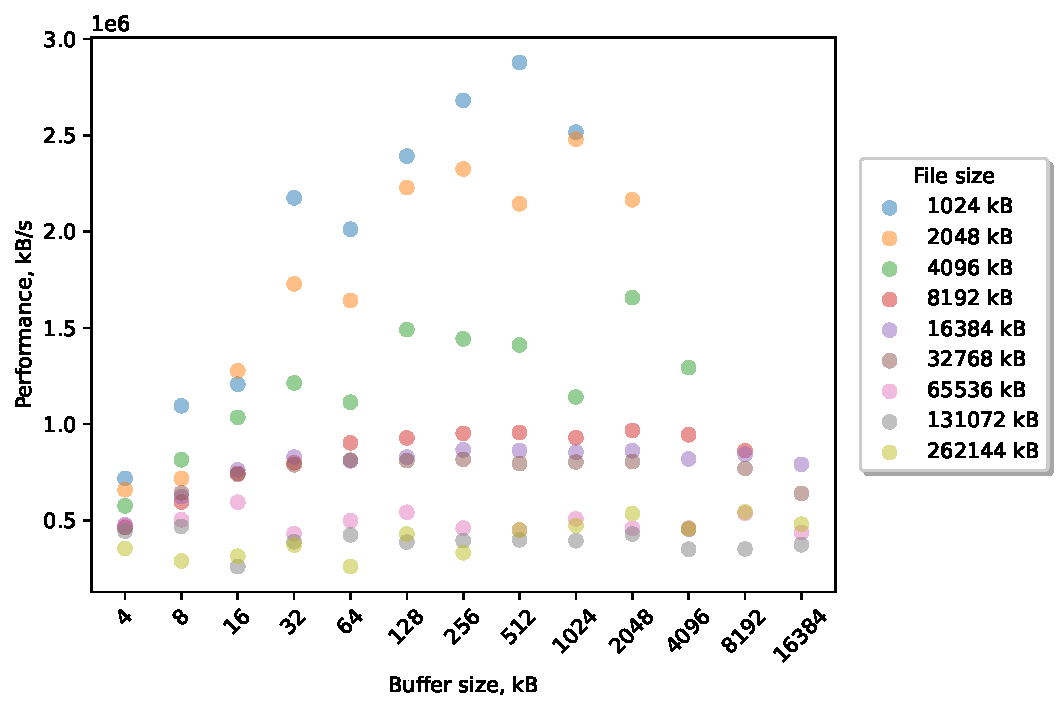
\includegraphics[width=1.0\textwidth]{figures.nosync/benchmarking/old/local/Re-Write.pdf}
% 	\end{center}
% 	\caption{IOZone output for \gls{APFS} \mbox{Re-Write}}
% \end{figure}

% \begin{figure}[!htb]
% 	\label{fig:bench_apfs_rnd_read}
% 	\begin{center}
% 		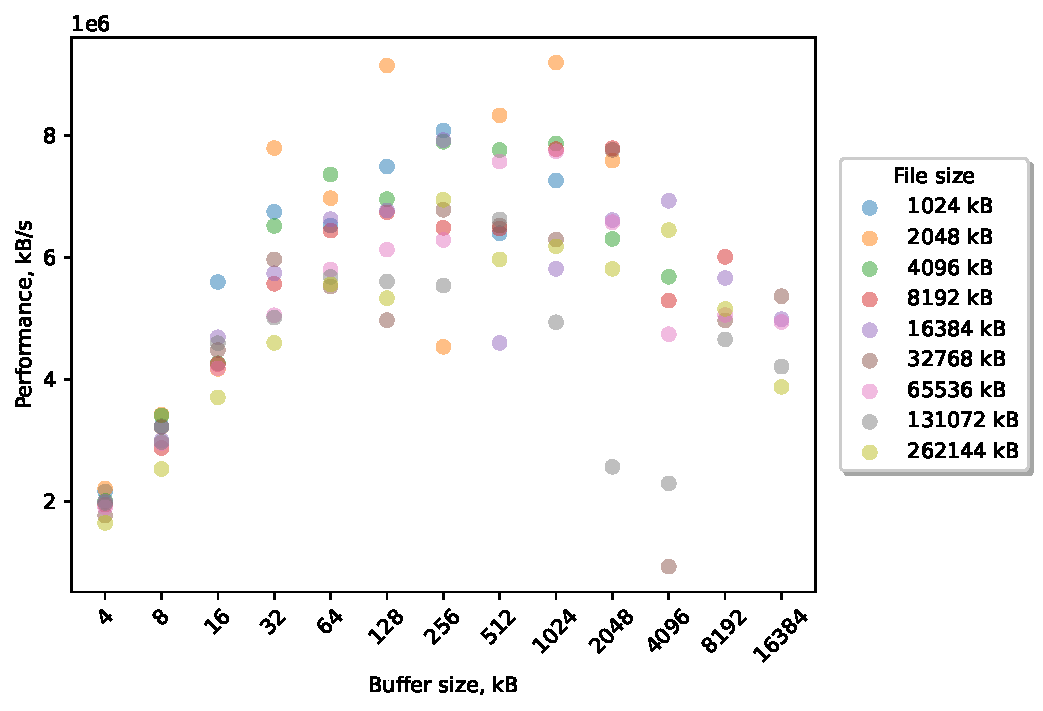
\includegraphics[width=1.0\textwidth]{figures.nosync/benchmarking/old/local/Random read.pdf}
% 	\end{center}
% 	\caption{IOZone output for \gls{APFS} Random read}
% \end{figure}

% \begin{figure}[!htb]
% 	\label{fig:bench_apfs_rnd_write}
% 	\begin{center}
% 		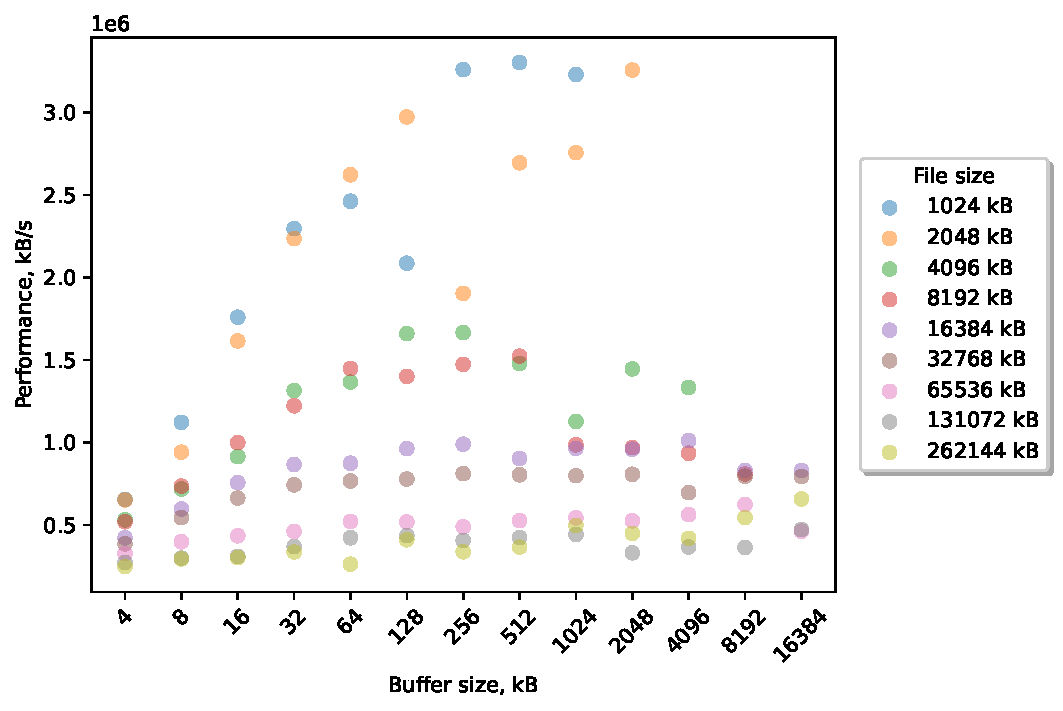
\includegraphics[width=1.0\textwidth]{figures.nosync/benchmarking/old/local/Random write.pdf}
% 	\end{center}
% 	\caption{IOZone output for \gls{APFS} Random write}
% \end{figure}